% The final version needs to be converted to word (or other related format)
% so there's no point in spending a huge amount of time getting everything
% looking perfect in this document.  But it will be much easier for us to
% collaborate with latex rather than word.
%
% Pages 10-15
% Due: 31 Dec 08 !!
% 
% Want lots of graphics and illustrative code samples
% All graphics need to work in black & white


\documentclass[oneside]{article}
\usepackage{fullpage}
\usepackage[pdftex]{graphicx}
\graphicspath{{graphics/}}
\DeclareGraphicsExtensions{.png,.pdf}
\usepackage{hyperref}
\usepackage{verbatim}
\renewcommand\rmdefault{bch}
\usepackage[small]{caption}
\usepackage[tiny]{titlesec}
\titlelabel{}
\linespread{1.07} 

\usepackage[round,sort&compress,sectionbib]{natbib}
\bibliographystyle{plainnat}

\title{Bay area blues: the effect of the housing crisis}
\author{Hadley Wickham, Deborah F. Swayne and David Poole}
\date{\today}

\raggedbottom

\begin{document}
\maketitle 

\section{Introduction}

The housing market has received a great deal of attention in the media for the past several years.  From about 2000 until 2006, we watched with excitement and apprehension as prices soared; since then, we've watched them tumble as credit became scarce and foreclosures mounted.   In this chapter, we take a closer look at this story by analyzing the sales of half a million homes in the San Francisco Bay Area from 2003 to 2008.  What can we learn about the way prices rose and fell throughout a single region and across a wide range of prices?

% We use a few simple statistical tools, but we place our primary focus on graphical displays of the data.  
% (Given that none of us live there, you might wonder why we chose to explore the Bay Area, but it revolves around the availability of the data.)

We begin by describing the data, how we obtained it, and how we prepared it for analysis by restructuring, transforming, cleaning, and augmenting the raw data.  As our analysis proceeds, we communicate most of our observations using graphical displays.  Along the way, we will also describe some of the tools we use, most of which are freely available.   Our main tool is R, a statistical programming and data analysis environment, and we used it at all stages: fetching, cleaning, analysis, diagnostics, and presentation.

% Let's come back to this after we have a finished conclusions section.
%
%We conclude by describing the interesting features that we uncovered, and we summarize what the data tell us about the housing crisis in the Bay area.

\section{How did we get the data?}

%Finding relevant datasets for a particular problem is challenging and requires a lot of exploration and investigation.  

Once we decided that we were interested in real estate sales, the search for data began.  Data searches are not always successful, so we felt particularly lucky when we found weekly sales of residential real estate (houses, apartments, condominiums, etc.) for the Bay Area produced by the San Francisco Chronicle, \url{http://www.sfgate.com/homesales/}.  We felt even luckier when we figured out that we didn't have to extract the data by parsing web pages, but that the data are already available in a machine-readable format.  Each human-readable (html web page) weekly summary is built from a text file that looks like this: 

\begin{verbatim}
rowid: 1
county: Alameda County
city: Alameda
newcity: 1
zip: 94501
street: 1220 Broadway
price: $509,000
br: 4
lsqft: 4420
bsqft: 1834
year: 1910
\end{verbatim}

The data for each week is available at a url of the form \url{http://www.sfgate.com/c/a/year/month/day/REHS.tbl}.  This is pretty convenient and only requires generating a list of all Sundays from the first on record, 2003/04/27 (which we found on the archive page), to the most recent, 2008/11/16 (at the time of analysis).  With this list of dates in hand, we then generated a list of urls in the correct format and downloaded them with the Unix command line tool {\tt wget}. We used wget because it can easily resume where it left off if interrupted.
% this saves a lot of time when you're moving from place to place on a laptop.

With all the data on a local computer, the next step was to convert the data into a standard format.  We often use the csv (comma separated values) format; it is easy to generate  csv files, and every statistical package (and Excel!) can read them.  We generated a csv file of the form:

\begin{verbatim}
county,city,zip,street,price,br,lsqft,bsqft,year,date,datesold
Alameda County,Alameda,94501,1220 Broadway,509000,4,4420,1834,1910,2003-04-27,NA
Alameda County,Alameda,94501,429 Fair Haven Road,504000,4,6300,1411,1964,2003-04
-27,NA
Alameda County,Alameda,94501,2804 Fernside Boulevard,526000,2,4000,1272,1941,200
3-04-27,NA
Alameda County,Alameda,94501,1316 Grove Street,637000,3,2700,1168,1910,2003-04-2
7,NA
\end{verbatim}

The original format may have been easier for a human to read, but this is easier for computers.  It is both more standard and more compact (45 megabytes instead of 90).  If you look closely at the sample data you might notice something that needs some explanation: the {\bf NA}s.  NA stands for not applicable, and is the sentinel value that R uses to represent missing values. We must take care to account for the missing values in our analysis.
%Missing values have special semantics which, by default, will propagate missingness throughout a summary: 5 + NA = NA, 5 < NA = NA and so on. We always need to make a deliberate decision to drop the missing values from an analysis.

It takes only a few minutes to parse the files for all 293 weeks and create {\tt house-sales.csv}, a csv file with 521,726 observations and 11 variables.  It took much more time to tweak the parser to get all the edge cases right: we needed to convert prices to regular numbers (by removing \$ and ,), parse the dates into a consistent format, and fill in missing values for fields that didn't occur in all of the tables. 

% it can take far longer to prepare the data in a consistent, machine-readable form than it takes to perform the actual analysis.
% HW: this wasn't the point I was trying to make (although I totally agree with it) - I was arguing that programming time out weighs computation time.  Speeding up computation by a factor of 10 wouldn't have that much effect on total analysis time, even for this very large data set)
%the time taken to compute the answer is totally overwhelmed by the time necessary to develop the correct approach.

% dfs- I now understand your point.  I can't find a concise way to express it, and I'm not sure taking the time to explain it fully is justified for the average reader.  What to do?  The paragraph stands nicely on its own.

\section{Geocoding} 

When we first looked at these data, we thought it would be really important to geocode all 436,106 unique addresses.  That is, we wanted to associate a latitude and longitude with each address so that it would be easy to explore fine-grained spatial effects. This is an interesting challenge: How can you geocode nearly half a million addresses? 
%In the end, we didn't end up using this extra data as much as we thought we would, but it is still an interesting challenge: how can you geocode nearly half a million addresses?  

We started by looking at the well-known web services provided by Google and Yahoo! These were unsuitable for two reasons: they impose strict daily limits on the number of requests, and there are cumbersome restrictions on the use of the resulting data.  The request limit alone meant that it would take well over a month to geocode all the addresses, and then the licensing would have affected publication of the results! After further investigation we found a very useful open service, the USC WebGIS, provided by the GIS research laboratory at the University of Southern California \citep{uscgis}.  This service is free for non-commercial use and makes no restrictions on the uses of the resulting data.  There was no daily usage cap when we began using the service, but there is an implicit cap caused by the speed: We could only geocode about 80,000 addresses per day, so it took us around 5 days to do all 400,000.  The disadvantage of this free service is that the quality of the geocoding is not quite as good (they use only publicly available address data), but the creators were very helpful and have published an excellent free introduction to the topic in \citet{goldberg:2008}.  

As well as latitude and longitude, the USC results also include a categorical variable indicating their degree of accuracy: exact address, zip code, county, etc.

% given the number of addresses I re-coded, I'd just as soon skip 
% most of this paragraph.  dfs
% 10\%  percent of the addresses were located exactly based on property boundaries (extremely accurate), another 75\% percent were located by interpolating between the numbers at each end of the block (very accurate), 7\% to the centre of the zip code (not very accurate) and the remainder were only located to the centre of the city or not at all.  

%       QUALITY_ADDRESS_RANGE_INTERPOLATION 75.30\%
%             QUALITY_EXACT_PARCEL_CENTROID  9.85\%
% QUALITY_ZIP_CODE_TABULATION_AREA_CENTROID  7.11\%
%       QUALITY_COUNTY_SUBDIVISION_CENTROID  0.12\%
%         QUALITY_UNIFORM_LOT_INTERPOLATION  0.04\%

\section{Data checking}

It is in general worth spending a significant amount of time at every stage of an analysis to make sure that data are accurate, and geocoding was no different.  Errors in geocoding came from a number of sources:  There are typographical errors in the addresses, new buildings are often not listed in public databases, and zip codes may be reassigned over time.  We further suspect that the USC software included a bug during the period we used it, because large numbers of addresses were falsely assigned to the Los Angeles area and elsewhere around the state; we remapped these addresses using another free on-line service at \url{gpsvisualizer.com}. Our debugging process included using R to draw simple maps of latitude vs. longitude for each county and most towns to identify the addresses that had been located far outside the Bay Area.

The addresses in San Jose posed an interesting geocoding challenge.  Sales are listed for several ``towns'' that are not recognized by any mapping sites we could find, so we assume they are informal names for neighbourhoods: North, South, East and West San Jose, Berryessa, Cambrian, and a few others.  

% This may be more than we need to say.

Where possible we tried to correct any errors.  When that was not possible, we used R's missing values to indicate that we do not know the exact latitude and longitude.  This is a better approach than throwing out bad matches, because we need varying levels of accuracy for different  purposes: When we map the data at the level of county or city, we can be satisfied with an approximate location.  The use of missing values for latitude and longitude ensures that any location with a suspicious geocoding will be dropped from analyses that use latitude and longitude, but included in all others.

\section{Analysis}

For a broad overview of the changes in the housing market, we'll start with the evolution of the average sale price and number of sales.  Since the data is reported weekly, that's a natural time unit to use.

% dfs:  check that the increase in weekly sales isn't an artifact of more towns and counties being reported in the Chronicle.
% Hadley removed the 4 counties for which we have no data before 2008; the trends were unchanged.

Figure~\ref{fig:daily} shows weekly average sale price and number of sales for the 293 weeks in the data.  There are some very interesting patterns.  The behavior of the average price is striking, with an increasing trend until June 2007 and then a precipitous drop to the present day ~--~ a clear illustration of the boom and bust in housing prices.  

Sales look quite different.  We see a seasonal effect, with fewer sales in the winter months. (This may be a good place to note that the data only rarely includes the true closing date, so we're using the date when the sale was reported in the newspaper, which may be four to six weeks later than the closing.)  Once we look past the seasonal effect, we see something else. Starting by the middle of 2006, sales volume decreases until early 2008, then suddenly begins to rise again. One possibility is that by this point house prices had dropped enough that buyers were shopping for bargains again; some of these could even be foreclosure sales.

\begin{figure}[htbp]
  \centering
    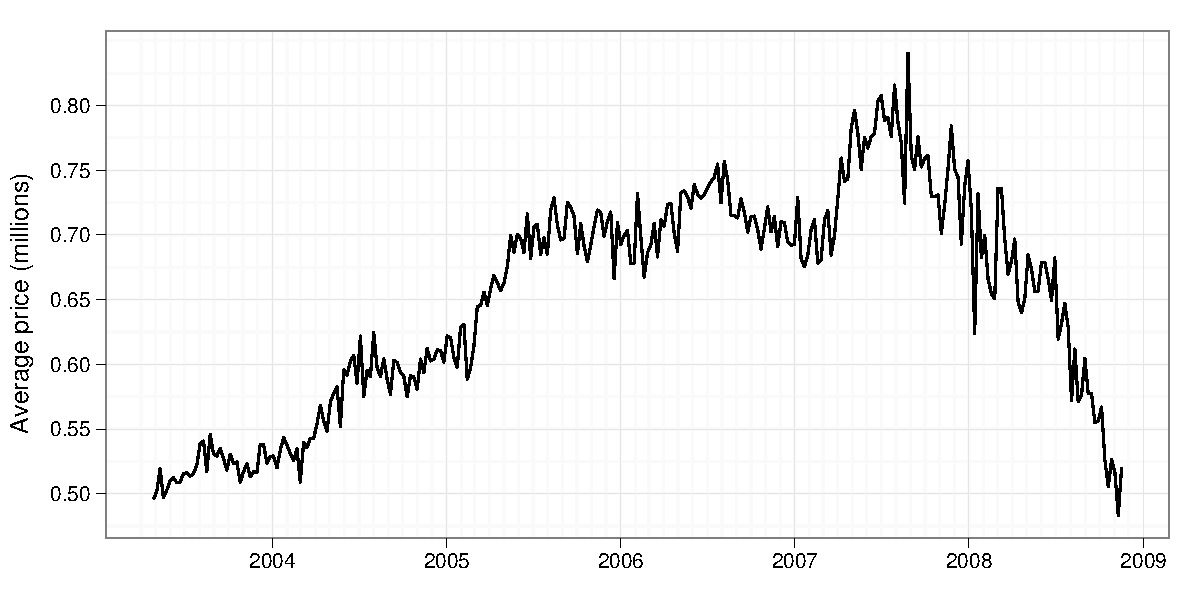
\includegraphics[width=0.5 \linewidth]{daily-price}%
    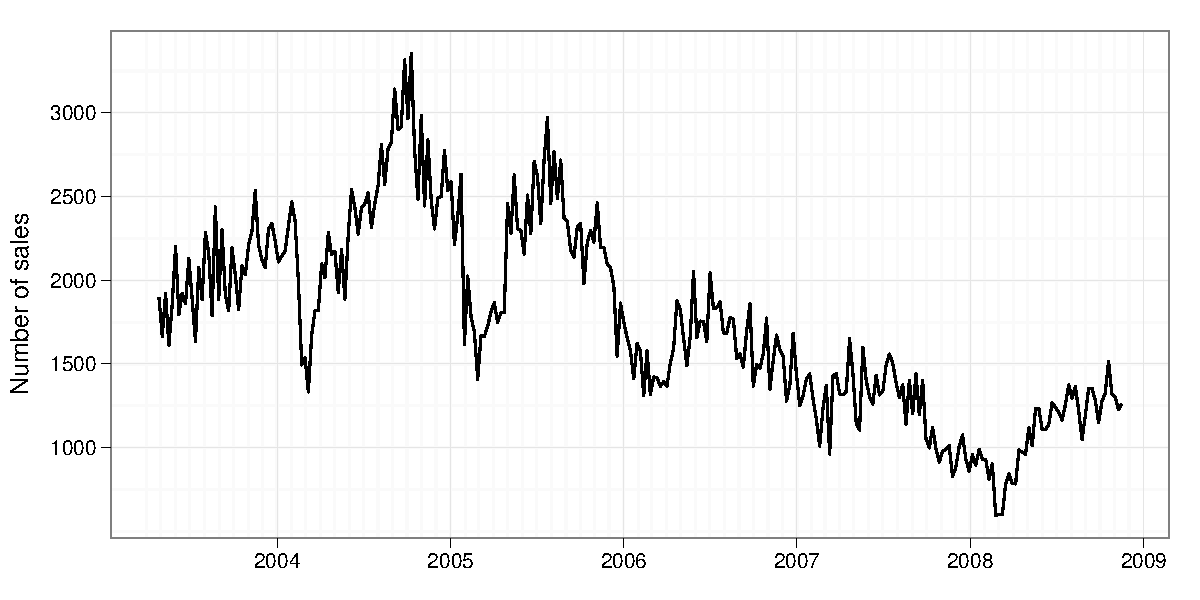
\includegraphics[width=0.5 \linewidth]{daily-sales}%
  \caption{Weekly average prices (left) and sales (right), showing clear evidence of the housing boom and bust.  Note, however, the uptick in sales in 2008.}
  \label{fig:daily}
\end{figure}

These simple plots suggest some directions for further exploration.  Are these patterns the same for homes in all price ranges?  What about different cities, or within neighbourhoods of a single city?  To investigate these questions, we'll follow roughly the same procedure:  We'll partition the data in different ways and compare the patterns for each partition.  We will create partitions based on house price (from most expensive to least) and physical location, both between cities and within a single city (San Francisco).

\subsection{The influence of inflation}
% explore-prices.r

Before proceeding with the analysis, though, we pause to consider inflation. The data were collected over a relatively short period of time (almost 6 years), but we wonder if we should adjust for inflation to ensure that the prices paid in 2003 are comparable to the prices paid in 2008.  A commonly used reference for calculating inflation is the consumer price index ({\sc cpi}) produced by the Bureau of Labor Statistics, \url{http://www.bls.gov/CPI}.  The {\sc cpi} calculates the price of a weighted ``basket'' of frequently purchased consumer goods and services.  This price is calculated monthly, and we will use the West coast series, series CUUR0400SA0, to adjust for inflation as follows.  We want to adjust all values to 2003 dollars, so we divide each {\sc cpi} value by its value in March 2003.  This operation is also known as indexing.  It gives the relative worth of a 2003 dollar at each point in time and makes it easy to read the effect of inflation from the graph: A value of 1.1 represents a cumulative inflation of 10\% from the start of the data.  
%Indexing is a very useful technique and we'll use it throughout our analysis.  
Figure~\ref{fig:inflation} shows the {\sc cpi}-based inflation measurement and the effect of adjusting prices for inflation.  Inflation has been steadily climbing over the last five years, and we can see that the inflation-adjusted rise in house prices is slightly less pronounced than the unadjusted trend. 

Finally, though, we decided not to adjust the sale prices for inflation. Housing prices have an influence on the {\sc cpi}, because one of its sub-indices is a housing index, a measure of rent and ``owner's equivalent rent.''  It could probably be argued that housing prices had a significant effect on the {\sc cpi} throughout the period under study.

\begin{figure}[htbp]
  \centering
    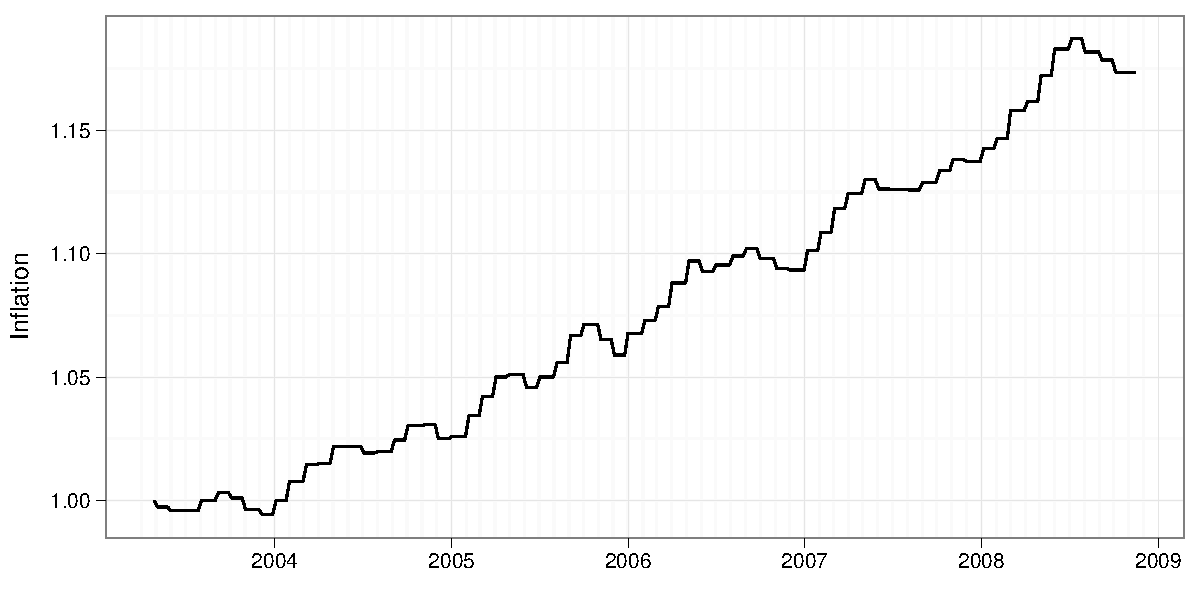
\includegraphics[width=0.5 \linewidth]{daily-cpi}%
    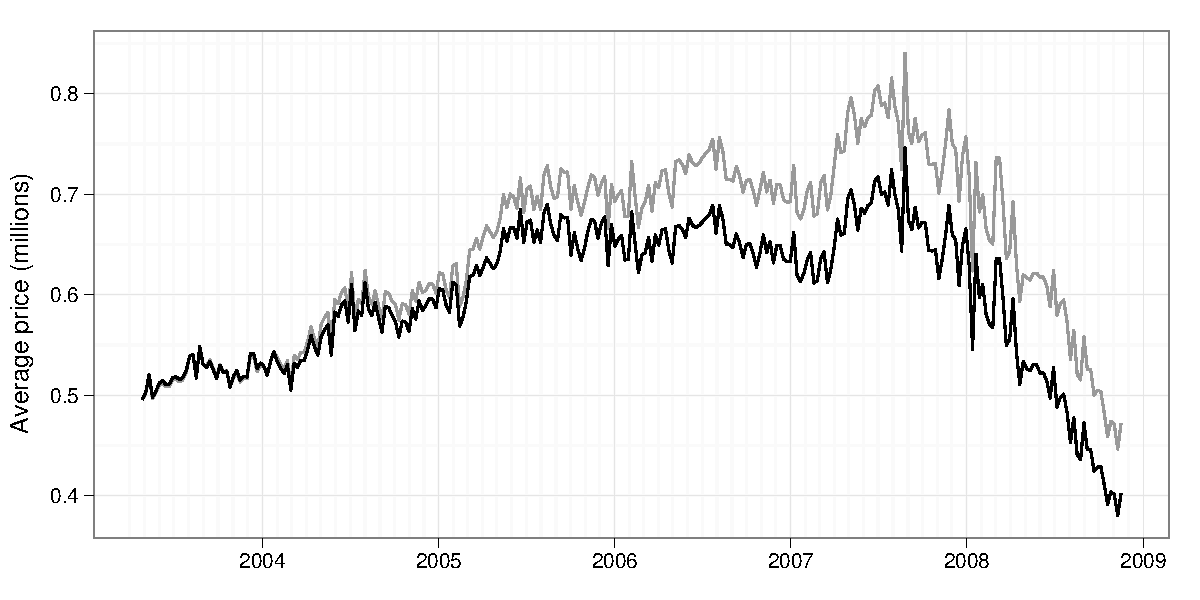
\includegraphics[width=0.5 \linewidth]{daily-price-adj}
  \caption{(Left) Inflation, indexed at 1 at start of series.  (Right) Inflation-adjusted house prices in 2003 dollars (black), and unadjusted prices (grey).  Failing to adjust for inflation makes the rise look a bit steeper, but has little effect on the decline. Monterey, San Benito, San Joaquin, and
and Santa Cruz counties excluded because we only have data for 2008.}
  \label{fig:inflation}
\end{figure}

With this basic overview in hand, we now drill down into the details. In the following sections we break the house sales into smaller groups, first by price and then by location.  We are interested in finding out whether the housing crisis has affected some groups of homeowners more than others.

\subsection{The rich get richer and the poor get poorer}
% explore-deciles.r

Has the housing crisis equally affected the rich and the poor?  Has the effect of the crisis been to improve or worsen the relative equality of these two groups?  In this section, we will explore how the crisis has affected the distribution of housing prices.  A big caveat is that we are looking at the Bay Area, so homes will be more expensive than in many other places in the country, but we still expect to see some relative inequalities.  (NB.  In the following, we will frequently use the word ``houses'' to refer to all categories of residential real estate: houses, townhouses, apartments, etc.)

As a first step, we calculate price deciles for each month.  The deciles are the nine prices for which 10\%, 20\%, 30\%, 40\%, 50\%, 60\%, 70\%, 80\%, and 90\% of houses cost less.  This is a succinct summary of the {\it distribution} of the prices for each month: instead of just looking at the average price, as we did earlier, we have nine numbers that summarise the complete distribution of the prices.   (We don't display the curves for the minimum or maximum price, because they would be too choppy.)

Figure~\ref{fig:decile-raw} shows how these deciles have changed over time.  The top line is the ninth decile, the price that 90\% of houses are less than, and the bottom line is the first decile, the price that only 10\% of houses are cheaper than.  The line in the middle is the median, the price which divides the houses into halves, half cheaper and half more expensive.  The lines are coloured from dark to light, from most to least expensive.  Each line follows a similar pattern, and we can see the effect of the housing bubble in mid 2007, particularly in the most expensive houses.  

\begin{figure}[htbp]
  \centering
  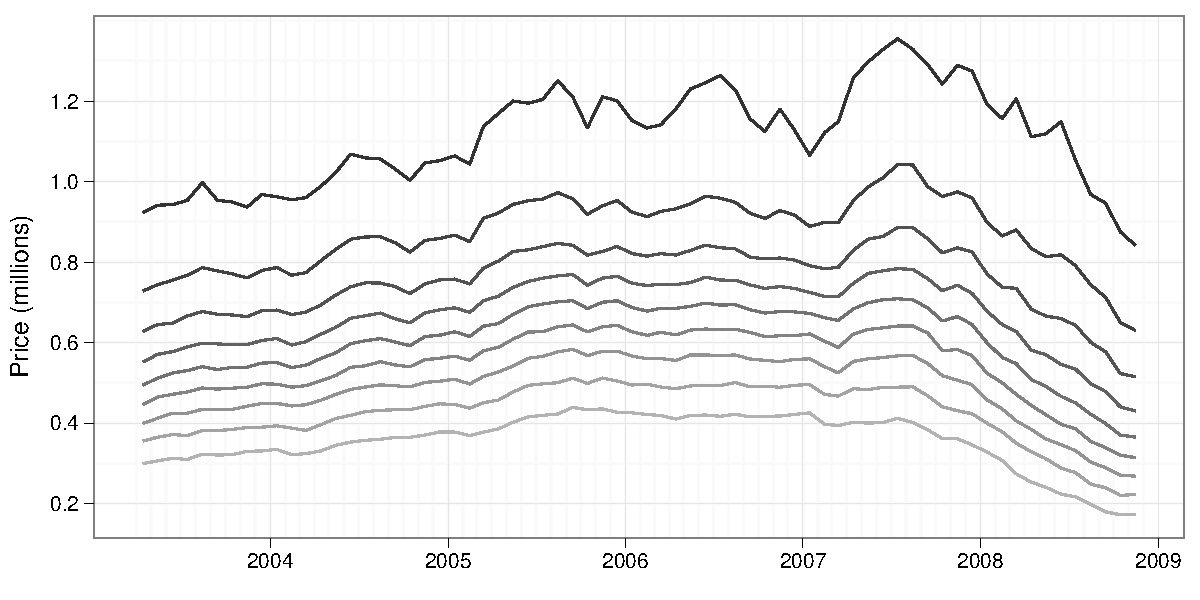
\includegraphics[width=0.75\linewidth]{decile-raw}
  \caption{Monthly average house price within each decile.  Lower deciles have lighter colours.  This plot clearly shows the nature of the bubble for the more expensive residences, but it is unrevealing about its effects at the lowest price ranges. } 
  \label{fig:decile-raw}
\end{figure}

This plot lets us compare the absolute values of each decile, but maybe it is more appropriate to look at the relative prices: How have the prices changed proportionately?  One way to look at the relative price is to compare each decile to its initial value.  To do this we index each decile, dividing each series by its initial price, just as we did for the {\sc cpi}. Figure~\ref{fig:decile-ind} shows these indices.  Each decile starts at 1.0 and we can see the relative change in price over time.  The interesting aspect of this plot is that the cheaper houses (the lighter lines) seem to peak higher and earlier (mid 2005), and then drop more rapidly thereafter. (Note the way the dark and light lines switch places in early 2007.) The cheapest houses, in the lowest decile, lost 43\% of their 2003 value compared to only 9\% for the most expensive houses. Comparing Figures~\ref{fig:decile-raw} and \ref{fig:decile-ind}, we see that although the biggest absolute decline in actual prices occurred at the expensive end, it was the cheapest houses that proportionately lost the most value. 

\begin{figure}[htbp]
  \centering
  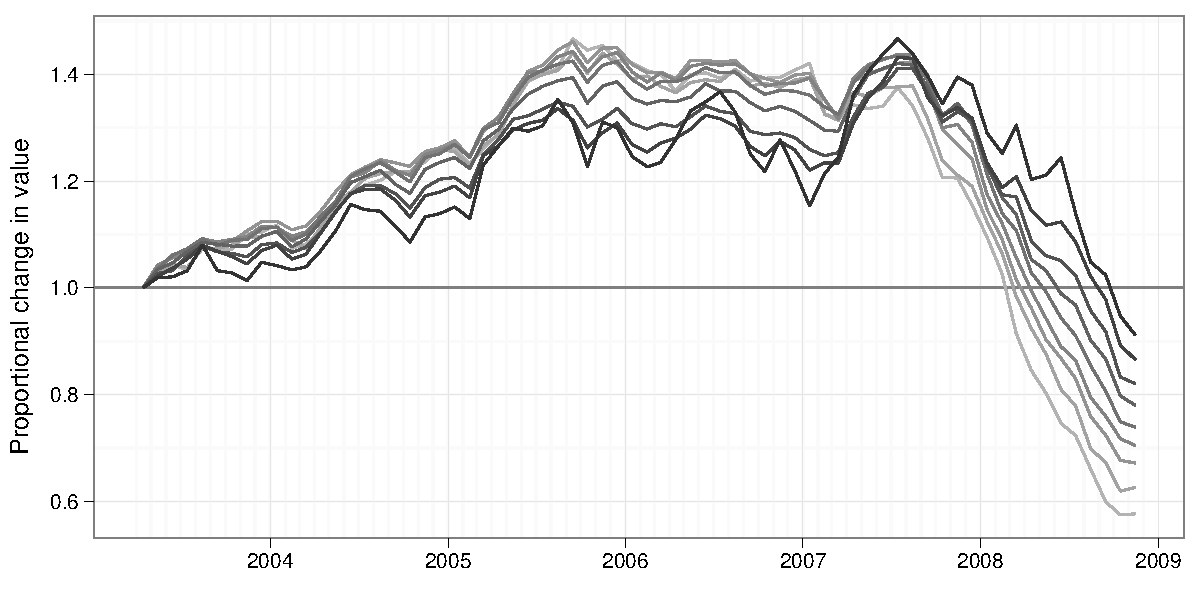
\includegraphics[width=0.75\linewidth]{decile-ind}
  \caption{Indexed house price within each decile. (The lighter the colour, the lower the price.)  The bust began earlier at the low end: The average price of less expensive houses peaked higher and earlier, and fell more steeply.}
  \label{fig:decile-ind}
\end{figure}

Another way to look at this inequality is Figure~\ref{fig:decile-rel}.  Here we have divided all the prices by the median price.  The values now represent a proportion of the median house price: A value of 1.2 represents a price 20\% higher than the median, and 0.8 is 20\% lower. Since the beginning of 2007, while the boom was still in full force at the high end, relative inequality has been growing.  Does this suggest that a widening of the price gap between expensive and cheap homes is a precursor to a subsequent crisis? Has this preceded other crises? These questions could be investigated further, but we don't have the data to pursue them here.

\begin{figure}[htbp]
  \centering
  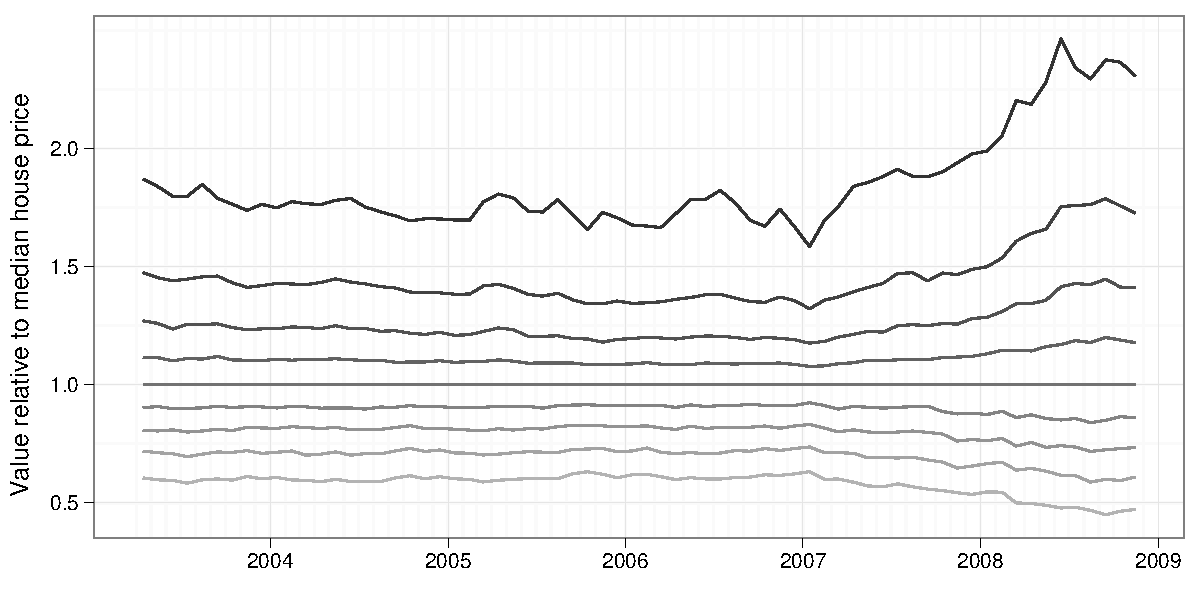
\includegraphics[width=0.75\linewidth]{decile-rel}
  \caption{House prices relative to the price of the median priced home.  The disparity in home prices has been increasing since early 2007.}
  \label{fig:decile-rel}
\end{figure}

\subsection{Geographic differences}
% explore-city.r

In this section we explore the changes in home prices in different cities in the Bay area.  Because we are looking at average prices, we must take care not to include cities with only a few sales. We decided to focus on all cities with an average of at least 10 sales per week. This gave us 58 cities (24\% of the 245 cities in the data) with 428,415 sales (82\% of the sales).  

We then calculated the average weekly house price. Figure~\ref{fig:spaghetti} shows these prices, with each city drawn with a different line.  Statisticians have an evocative name for this type of display: the spaghetti plot.  It's very hard to see anything in the big jumble of lines.  One method of improvement is to smooth each line, removing short-term variation and allowing us to focus on the long-term trends we are looking for.

\begin{figure}[htbp]
  \centering
    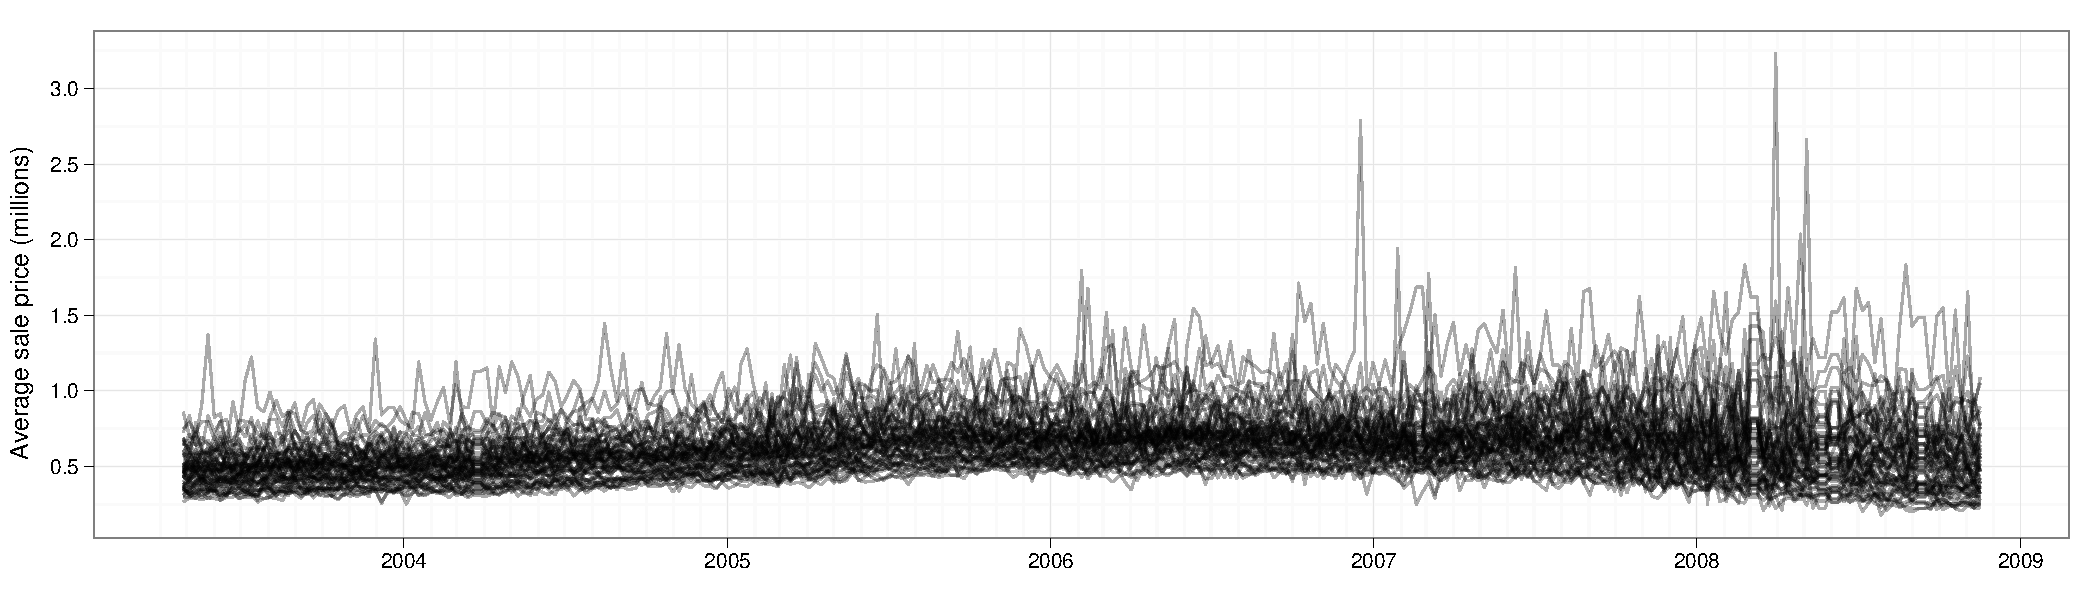
\includegraphics[width=0.9\linewidth]{cities-price}
  \caption{Average sale price for each week for each city.  This type of plot is often called a spaghetti plot.  It suggests the need for smoothing, because the week-to-week variation in the curves makes it impossible to detect trends.}
  \label{fig:spaghetti}
\end{figure}

To create smooth curves, we used generalised additive models ({\sc gam}), a generalisation of linear models \citep{wood:2006}.  This method fits smooth curves by optimising the trade off between being close to the data and being very smooth, in effect removing noisy short-term effects and to emphasizing the long-term trend.  This is exactly what we need: we are not interested in daily or weekly changes, only the long-term changes related to the housing crisis.

The left part of Figure~\ref{fig:smoothed} shows the result of this smoothing. This is a big improvement and we can now actually see some patterns! Note the big difference in scales between this plot and the first: smoothing the data has removed the large spikes which represent the sales of a few very expensive houses. We will also index each city in the same way we indexed each decile: dividing by the starting price puts each city onto a common scale and allows us to focus on the changes.  This is shown on the right of Figure~\ref{fig:smoothed}.  

\begin{figure}[htbp]
  \centering
  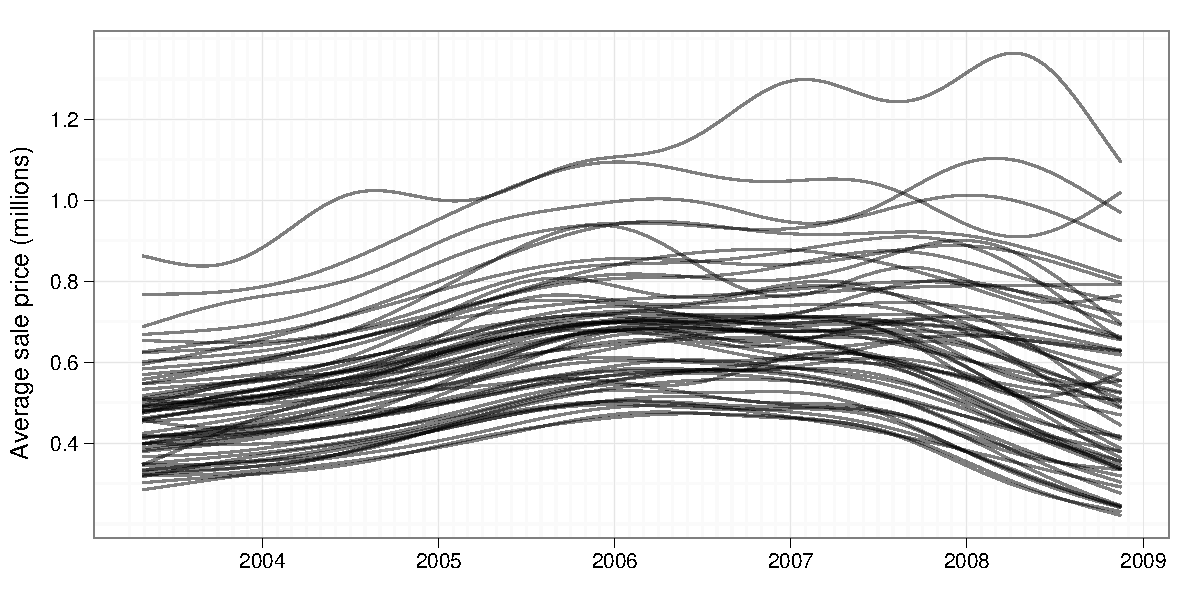
\includegraphics[width=0.5 \linewidth]{cities-smooth}%
  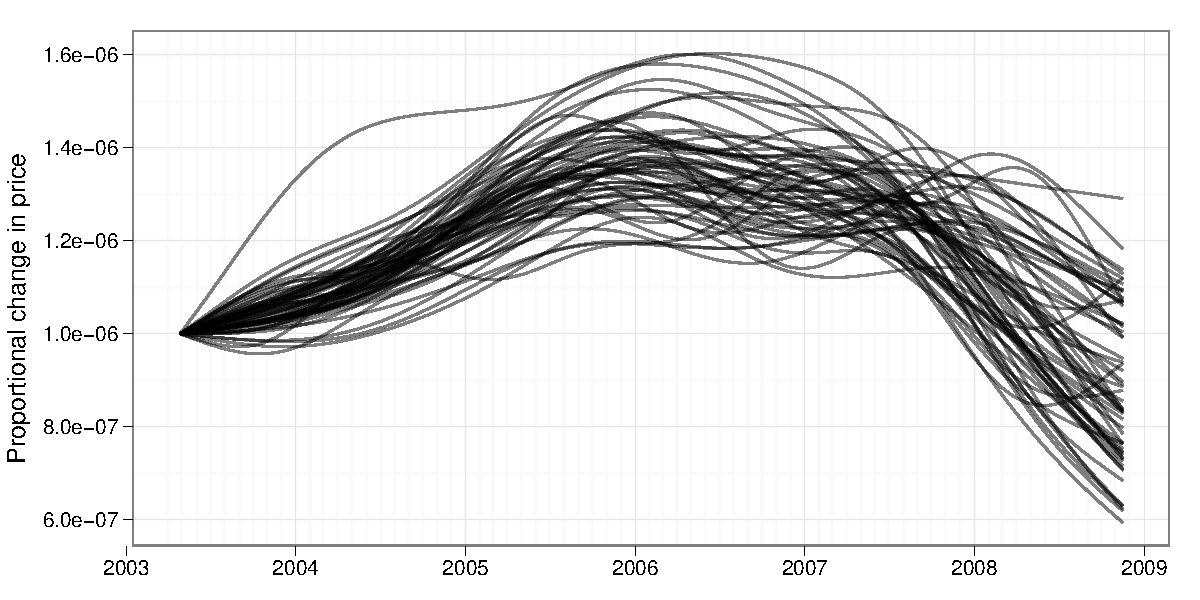
\includegraphics[width=0.5 \linewidth]{cities-indexed}
  \caption{Smoothed weekly average sale prices, one curve for each city (left).  The curves in the plot at right have been indexed to show proportional changes in price.  Patterns are beginning to emerge.}
  \label{fig:smoothed}
\end{figure}

There is a still a lot of variation, but we can start to see a pattern of increasing values until mid 2007, and then decreasing values afterwards.  To get any further, we need to look at the cities individually, as in Figure~\ref{fig:individual}.  This plot takes up a lot of space but is worthwhile for the extra information it affords.  We can pick out some interesting patterns: Berkeley and San Francisco show less of a peak and less of a drop, and Mountain View is unique in that it has seen no drop at all in housing prices.  Other cities such as Oakley, Vallejo, and San Pablo, show both big peaks and big drops.

Recall that in our earlier discussion about San Jose, we noted that the raw data describes many neighbourhoods of San Jose as cities in their own right.  Because of this, it sometimes happens that the same address is assigned to more than one neighbourhood, but this data suggests that the neighbourhoods have distinct characters.  Berryessa, East San Jose, North San Jose, and South San Jose have similar curves, showing a sharp peak and an equally sharp drop;  Cambrian, San Jose, and West San Jose, on the other hand, don't show much of a decline.

\begin{figure}[htbp]
  \centering
  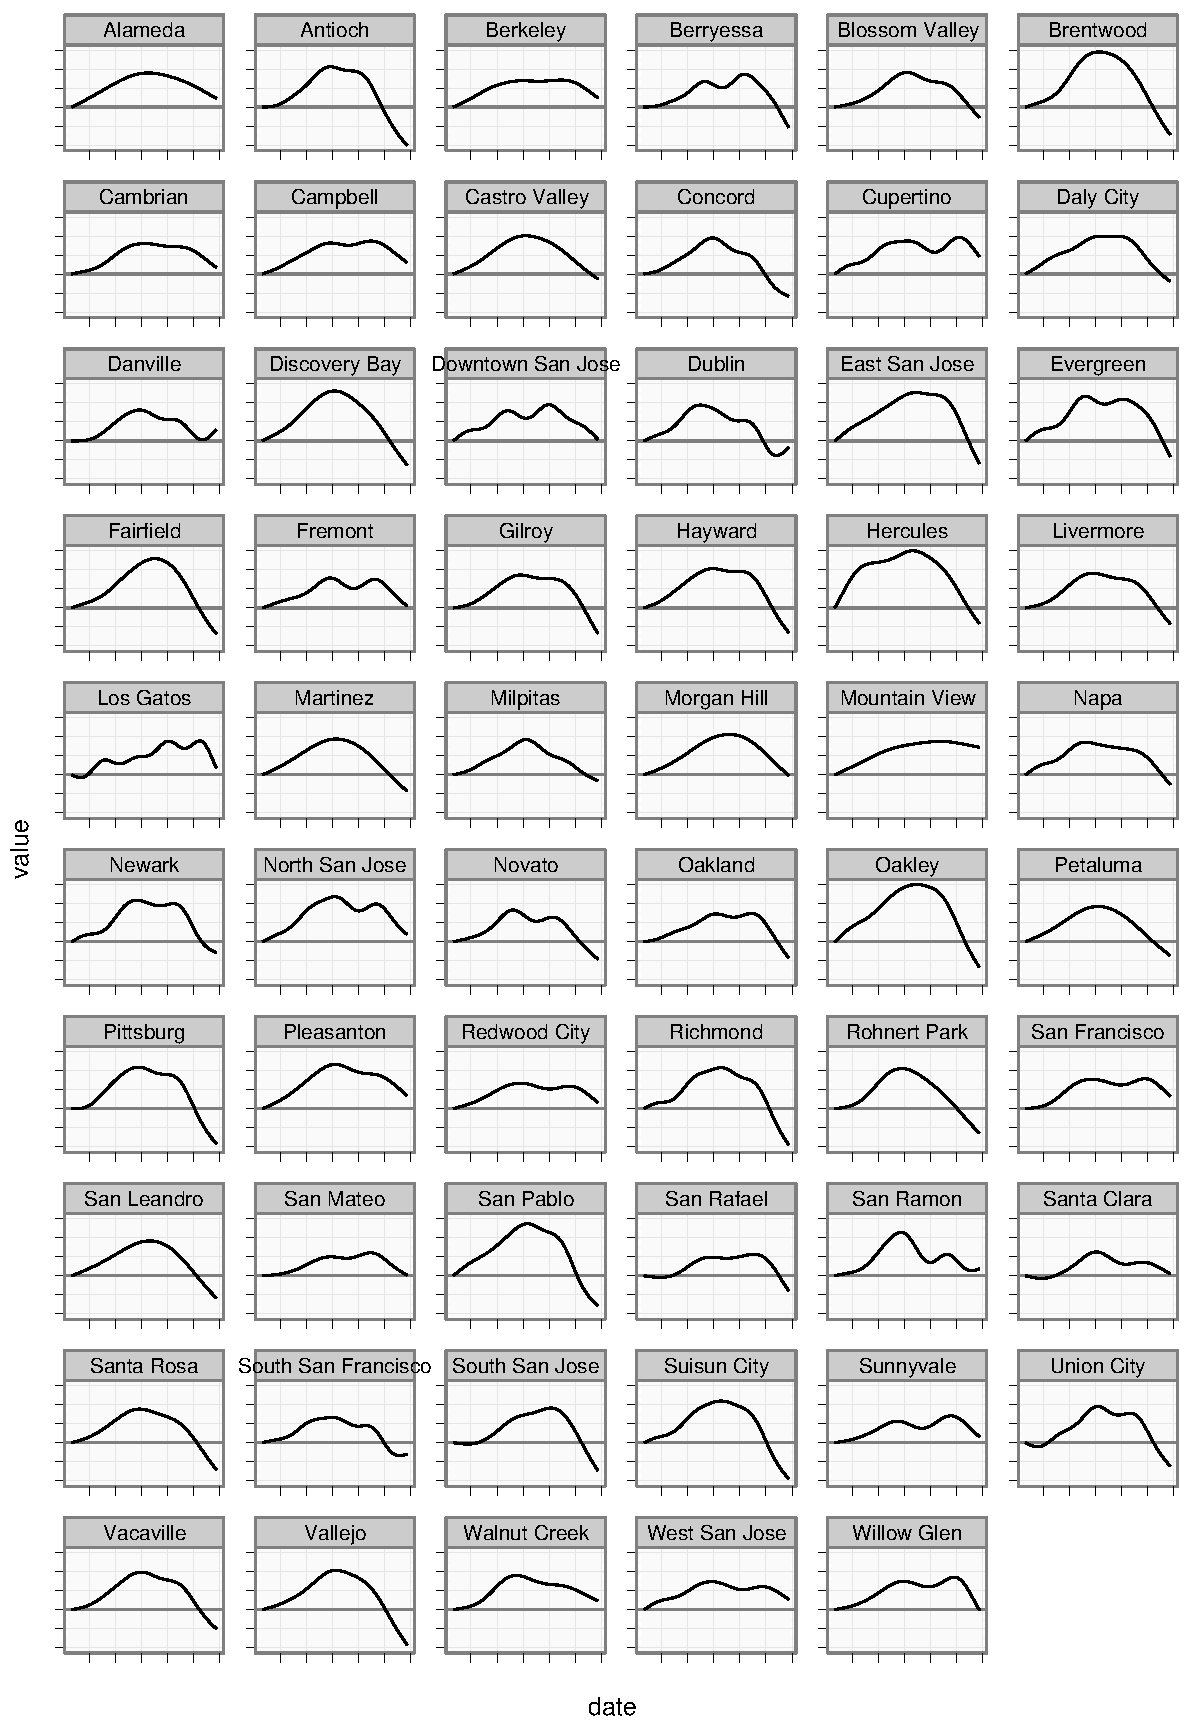
\includegraphics[width=0.9\linewidth]{cities-individual}
  \caption{Individual plots of the sales price for each city, smoothed and indexed.  These are exactly the curves that were plotted on top of one another in the previous figure (right).  San Pablo's curve shows the boom and bust of the housing market; Berkeley's curve shows less variation; Mountain View seems to be the only city where prices continue to rise. }
  \label{fig:individual}
\end{figure}

% Figure~\ref{fig:clustering} shows one way of clustering the cities into three groups.  Note how the groups are basically formed along the diagonal: it's the difference between the peak and the plummet that seems to be telling us the most.  Figure~\ref{fig:clustered} shows the result of the clustering, with each of the three groups displayed in its own panel.  The groups are somewhat arbitrary (we could shift the boundaries a little in either direction and have little effect)
% 
% \begin{figure}[htbp]
%   \centering
%     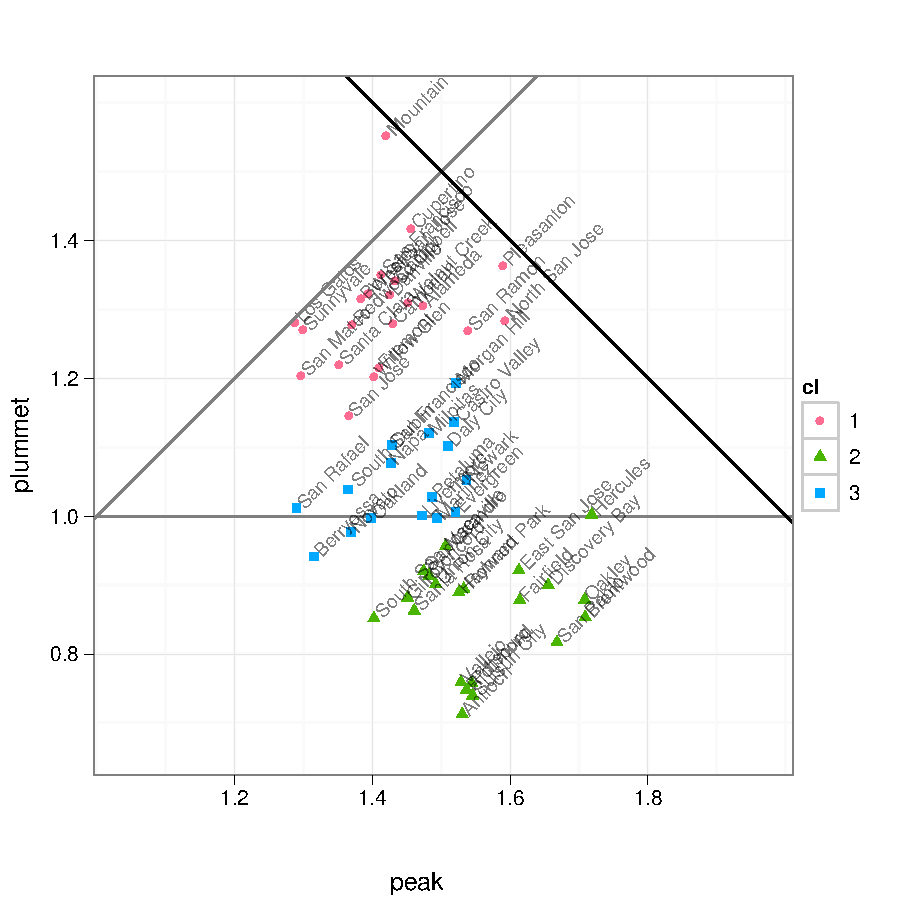
\includegraphics[width=0.7 \linewidth]{cities-clustering}
%   \caption{A scatterplot of cities with height at peak on x axis, and most recent value (plummet) on y axis.  The cities have been clustered into three groups.  The closer a city is to the line in the top left corner, the less the effect of the housing crisis on average prices.}
%   \label{fig:clustering}
% \end{figure}
% 
% \begin{figure}[htbp]
%   \centering
%   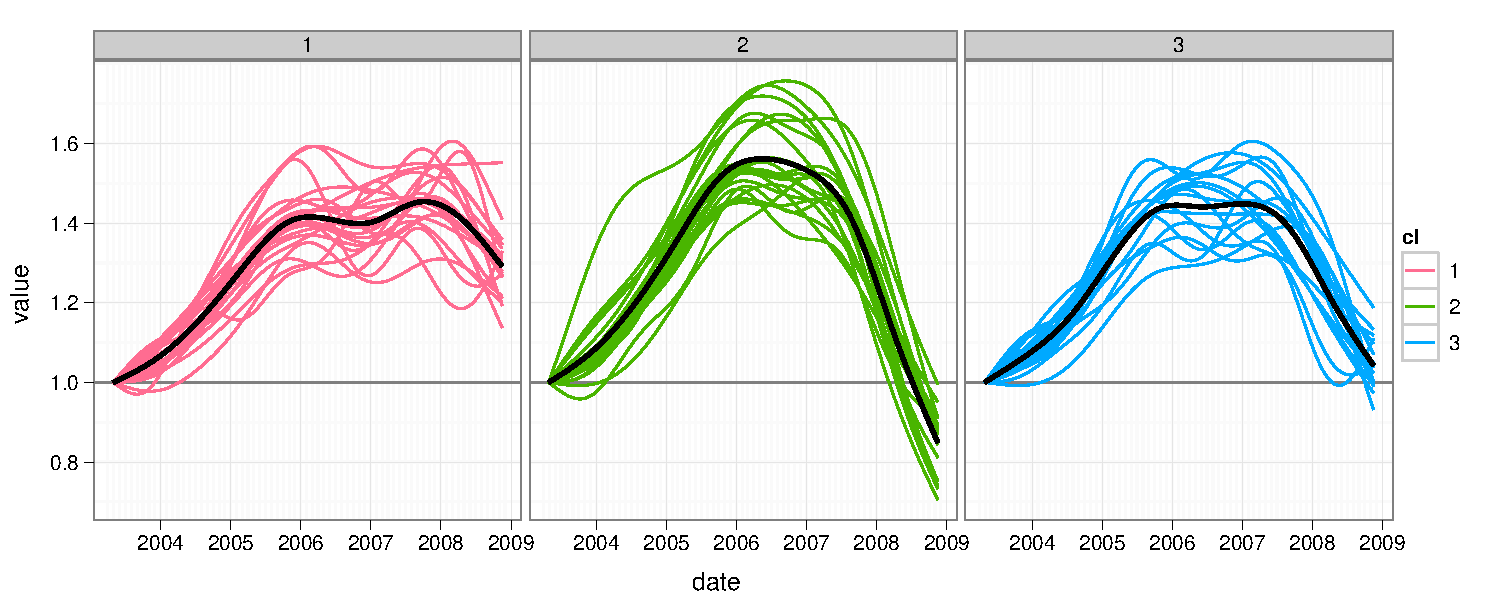
\includegraphics[width=\linewidth]{cities-indexed-clustered}
%   \caption{The index sale price time series for the three clustered identified in Figure~\ref{fig:clustering}.  Cluster one includes cities with low peak and no plummet, cluster two cities with high peak and big plummet, and cluster three is somewhere in between.  The thick lines represent smoothed patterns within each cluster.}
%   \label{fig:clustered}
% \end{figure}

After further investigation we concluded that there was one main feature that seemed to distinguish the different cities: the difference between prices at the peak of the boom and the depth of their most recent plummet.  We created a new variable called {\em price drop}, which is the relative decrease in average price between February 2006 (at the height of the boom) and November 2008 (the doldrums at the time of writing). Figure~\ref{fig:groups} groups the cities by this new variable.  The divisions are arbitrary, but one can see how the cities in each group follow a similar pattern: The bigger the boom, the bigger the collapse.  This suggests that this single number does a good job of summarising the boom-and-bust aspect of the housing crisis.

\begin{figure}[htbp]
  \centering
    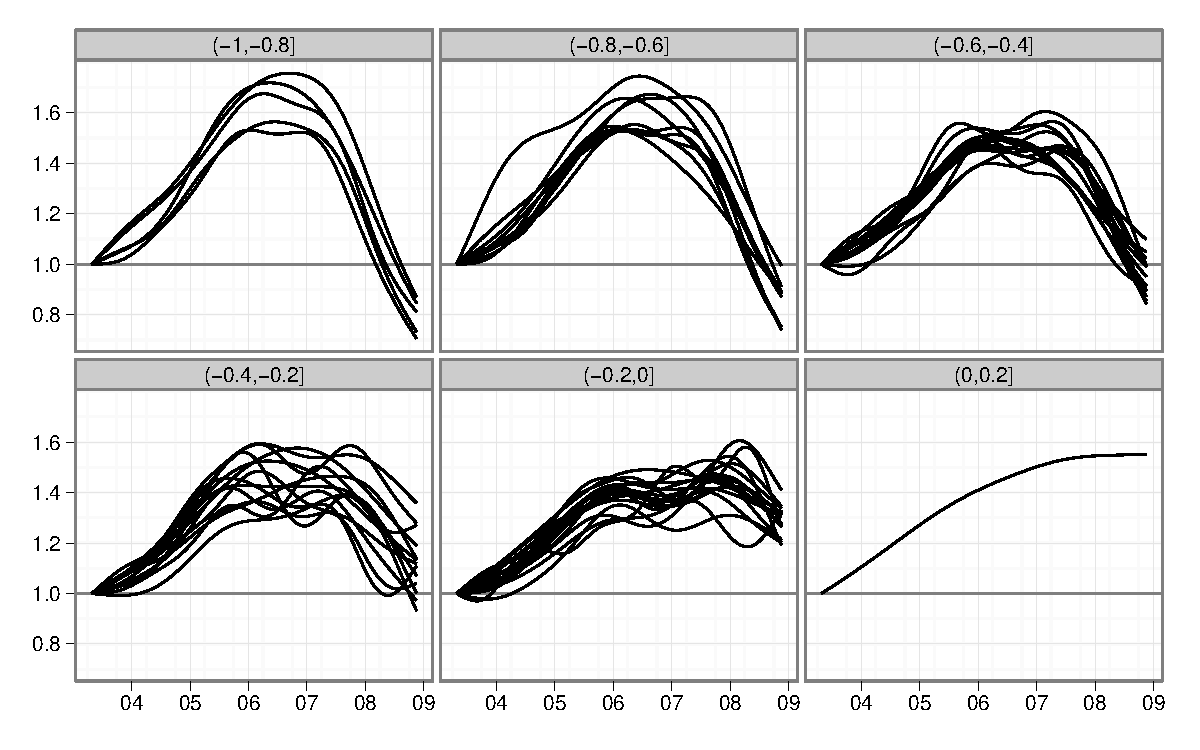
\includegraphics[width=0.75\linewidth]{cities-indexed-grouped}
  \caption{Plots grouping the curves for towns by their value of {\em price drop}.  The towns in the upper left plot had the largest price declines (between .8 and 1, or 80\% and 100\%); the town at the lower right (Mountainview) is the only one that shows no decline.  The patterns within each group are similar, suggesting that this single number provides a useful way to divide the cities into groups.}
  \label{fig:groups}
\end{figure}

We have determined that cities have different patterns, but we don't yet know why that might be so.  The geographic pattern, as in Figure~\ref{fig:geo} does not reveal anything particularly striking except that the worst hit towns tend to be to the north and the east. This does not offer much in the way of explanatory power, so we looked for additional data that might help us gain a deeper understanding. 

\begin{figure}[htbp]
  \centering
    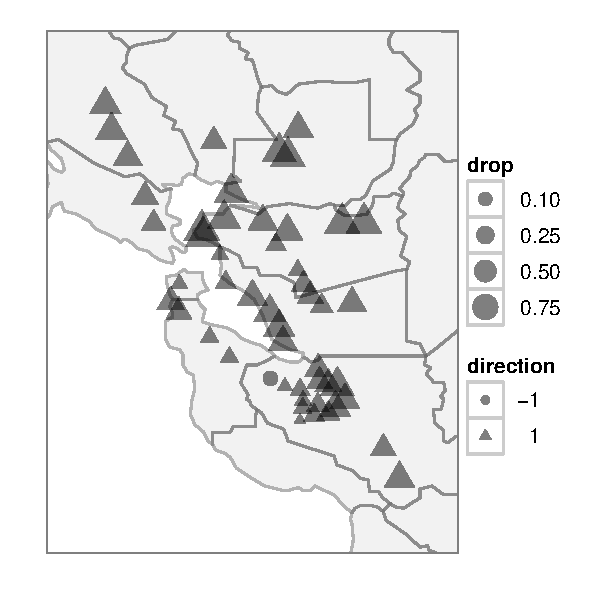
\includegraphics[width=0.5\linewidth]{cities-geo-changes}
  \caption{The geographic distribution of {\em price drop}.  The worst hit towns tend to be to the north and the east. The single triangle represents the location of Mountainview, the only city where the sale price has continued to increase. }
  \label{fig:geo}
\end{figure}

\section{Census information}

The US Census Bureau provides demographic data from recent surveys at both the county and city levels. The quickfacts website, e.g.,\ \url{http://quickfacts.census.gov/qfd/states/06/0649670.html}, displays a number of interesting demographic variables for each city. Unfortunately, city-level data are not available in an easily downloadable format, but we were able to use scripting methods (like those we used for the sales data) to collect the demographic information and convert it into csv.  In addition, the definition of a city differed slightly between the census data and the sales data, so we could only match 46 out of the full 58 cities.  The census data didn't cover some of cities we chose because their population was below some cutoff, and some of what the housing data calls ``cities'' are actually neighbourhoods within larger cities, as we noted earlier with respect to San Jose.

\begin{figure}[htbp]
  \centering
  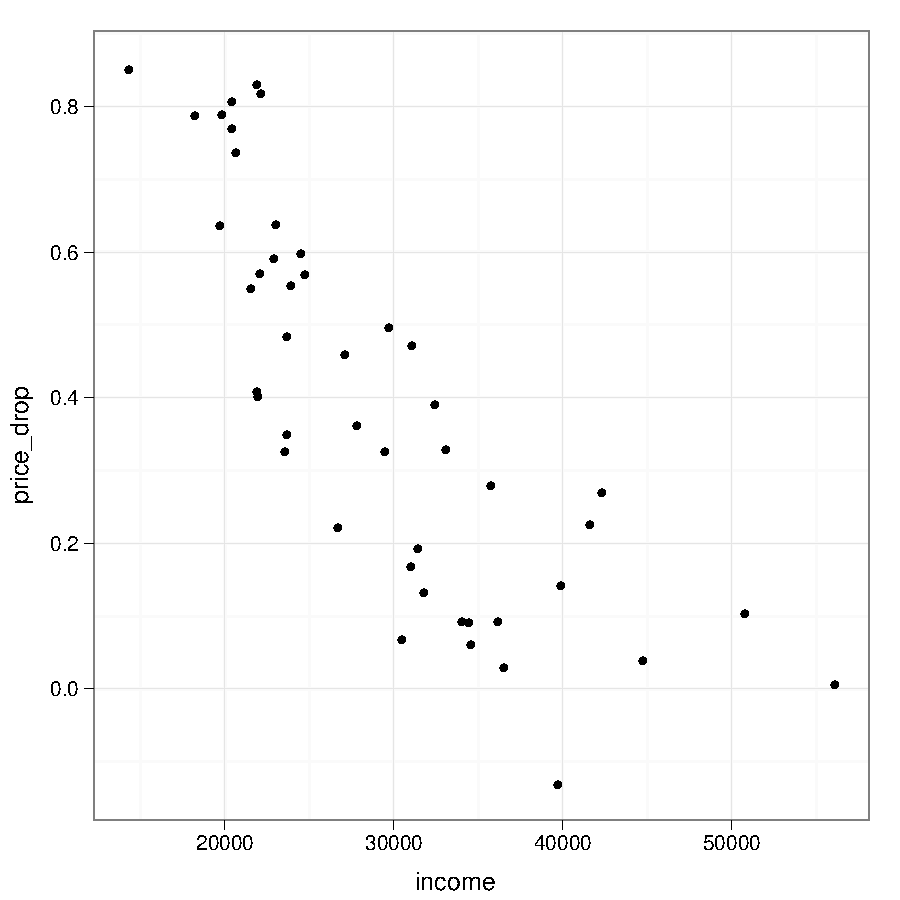
\includegraphics[width=0.33\linewidth]{cities-income}%
  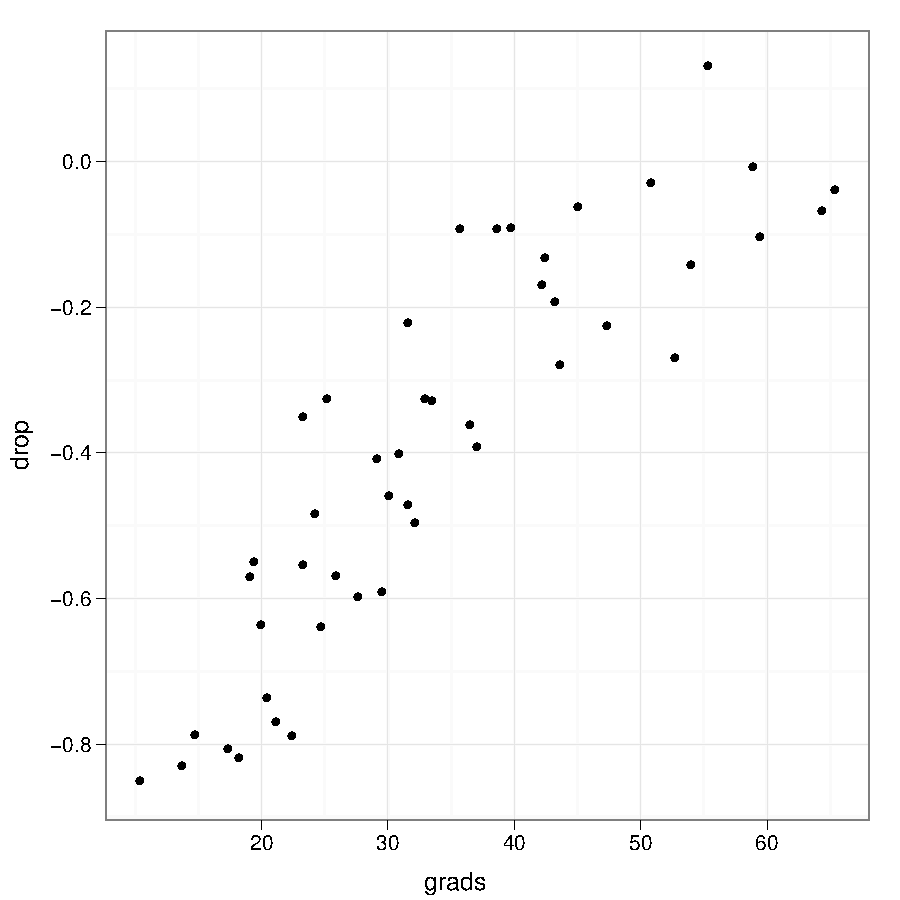
\includegraphics[width=0.33\linewidth]{cities-grads}%
  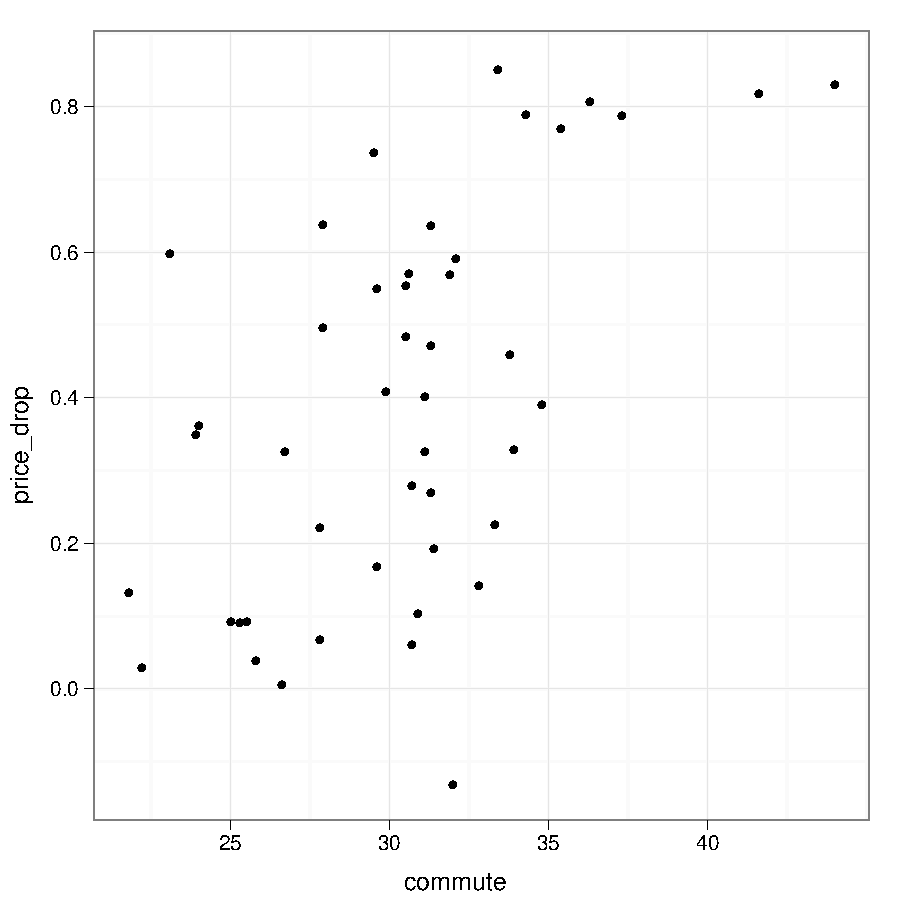
\includegraphics[width=0.33\linewidth]{cities-commute}
  
  \caption{From left to right, the relationship between the decline in house prices ({\em price drop}) and average income, percentage of college graduates and average commute time.}
  \label{fig:census}
\end{figure}

A glance at the demographic variables revealed that the most affected cities have a high percentage of babies and children, bigger households, fewer bachelors degrees, and longer commutes.  Most significantly these cities also have lower average incomes, which is probably the factor that drives many of the other relationships. Figure~\ref{fig:census} includes three scatterplots that illustrate the relationship between the drop in home prices and income, percentage of college graduates, and commute time.  The correlation between {\em price drop} and commute time is weak, but note that all of the cities with the longest commute times (more than 35 minutes) have particularly large drops in price. It appears that the housing crisis has been relatively more damaging in poorer areas.

The county-level census data contains more variables than the data for cities, so we analysed the county data for further explanation of the housing crisis. The plot on the left in Figure~\ref{fig:newconstruct} shows, for each county in which we had sales data, the percentage change in the number of housing units (from 2000 to 2006) plotted against the median sale price in 2008. There is a strong negative relationship between recent home values and the amount of new construction. In other words, most of the building boom in recent years occurred in poorer neighbourhoods, and as we noted above, these are also the areas where the subsequent slump has been the most severe. San Joaquin county, in particular, which has consistently low prices across towns, experienced by far the most new construction in recent years.  We should note that we do not have many sales in a few of these counties (e.g., San Benito and Santa Cruz), but the overall nature of this relationship is still very clear.  The effect is further illustrated by the right hand plot in Figure~\ref{fig:newconstruct}, which again shows the percentage change in housing units from 2000 to 2006, but this time plotted against the 2005 per-capita income at the county level, obtained from the census data. We notice the similarity to the previous plot, and it illustrates again that the intensity of new construction was higher in less affluent areas, even when aggregated across cities to the county level. It is clear too that prices and income are strongly positively correlated, which we observed at the city level in Figure~\ref{fig:census}.

%The effect is further illustrated in the right-hand plot in Figure~\ref{fig:newconstruct}, which shows the median price for all the sales in each year, as well as the median sale price for the subset of homes built in that year (and then sold in that year or later). We see that despite the large overall boom from 2003 to 2006, the new construction during this period was aimed increasingly at the lower end of the market.  

\begin{figure}[htbp]
  \centering
    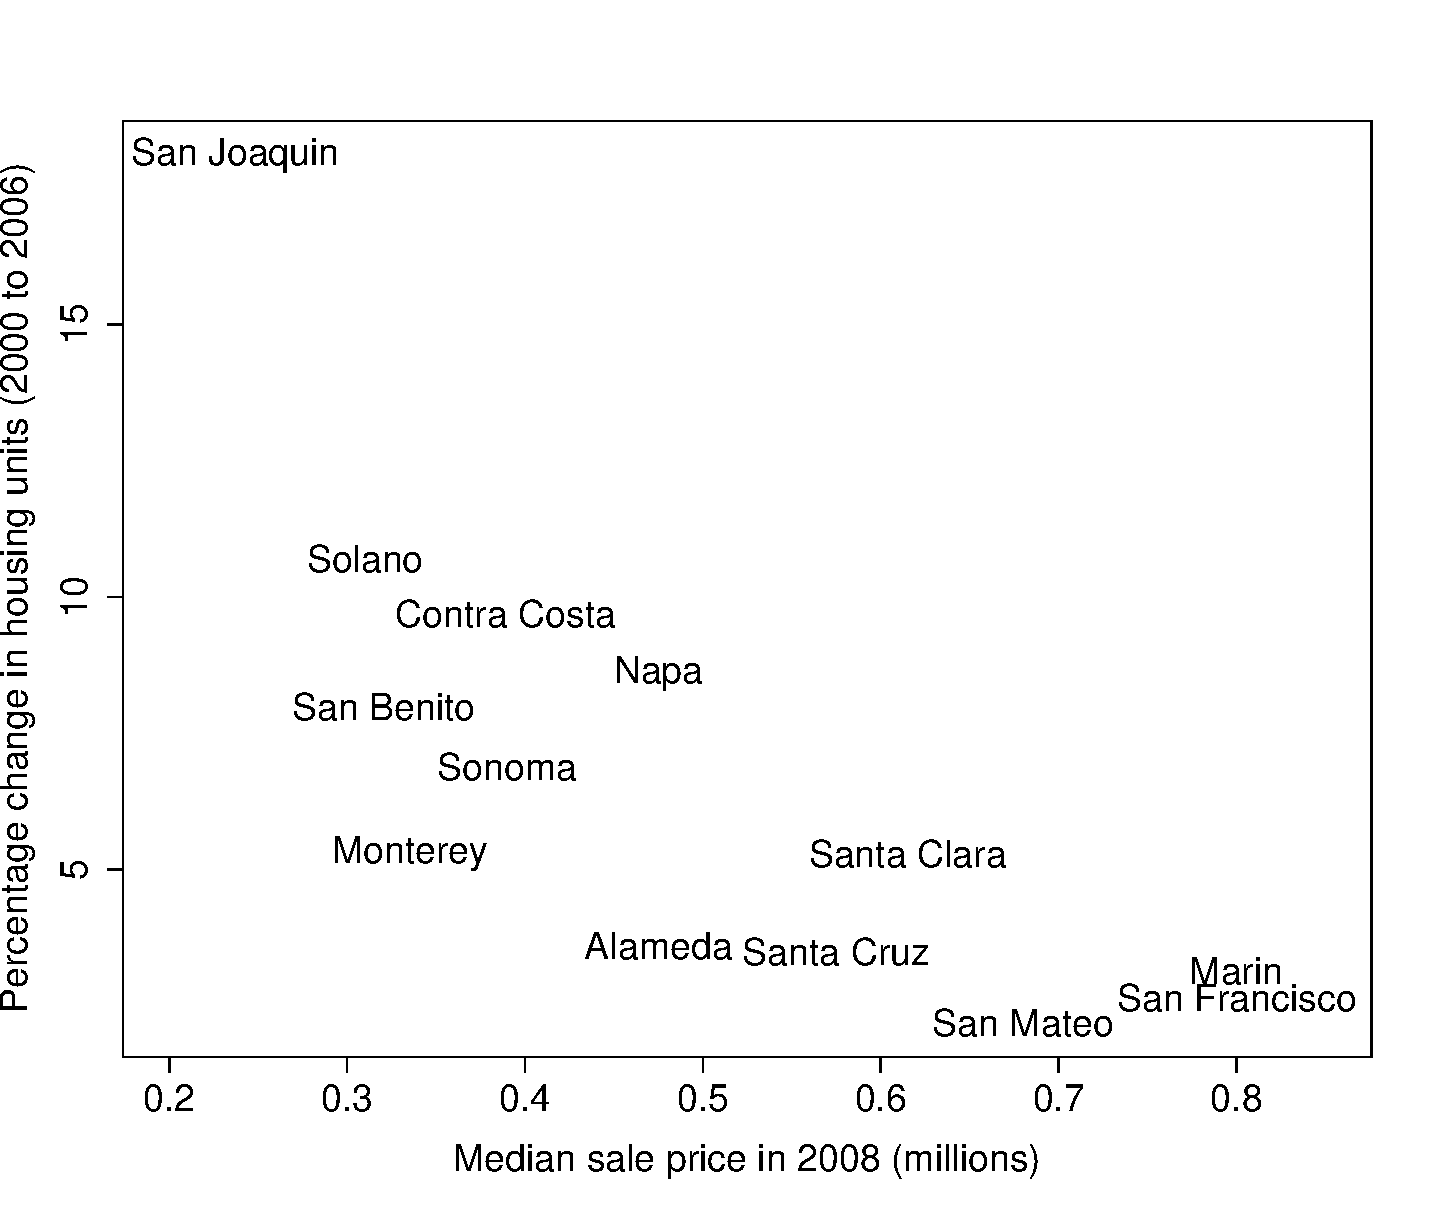
\includegraphics[width=0.5\linewidth]{county_newconstruct}%
    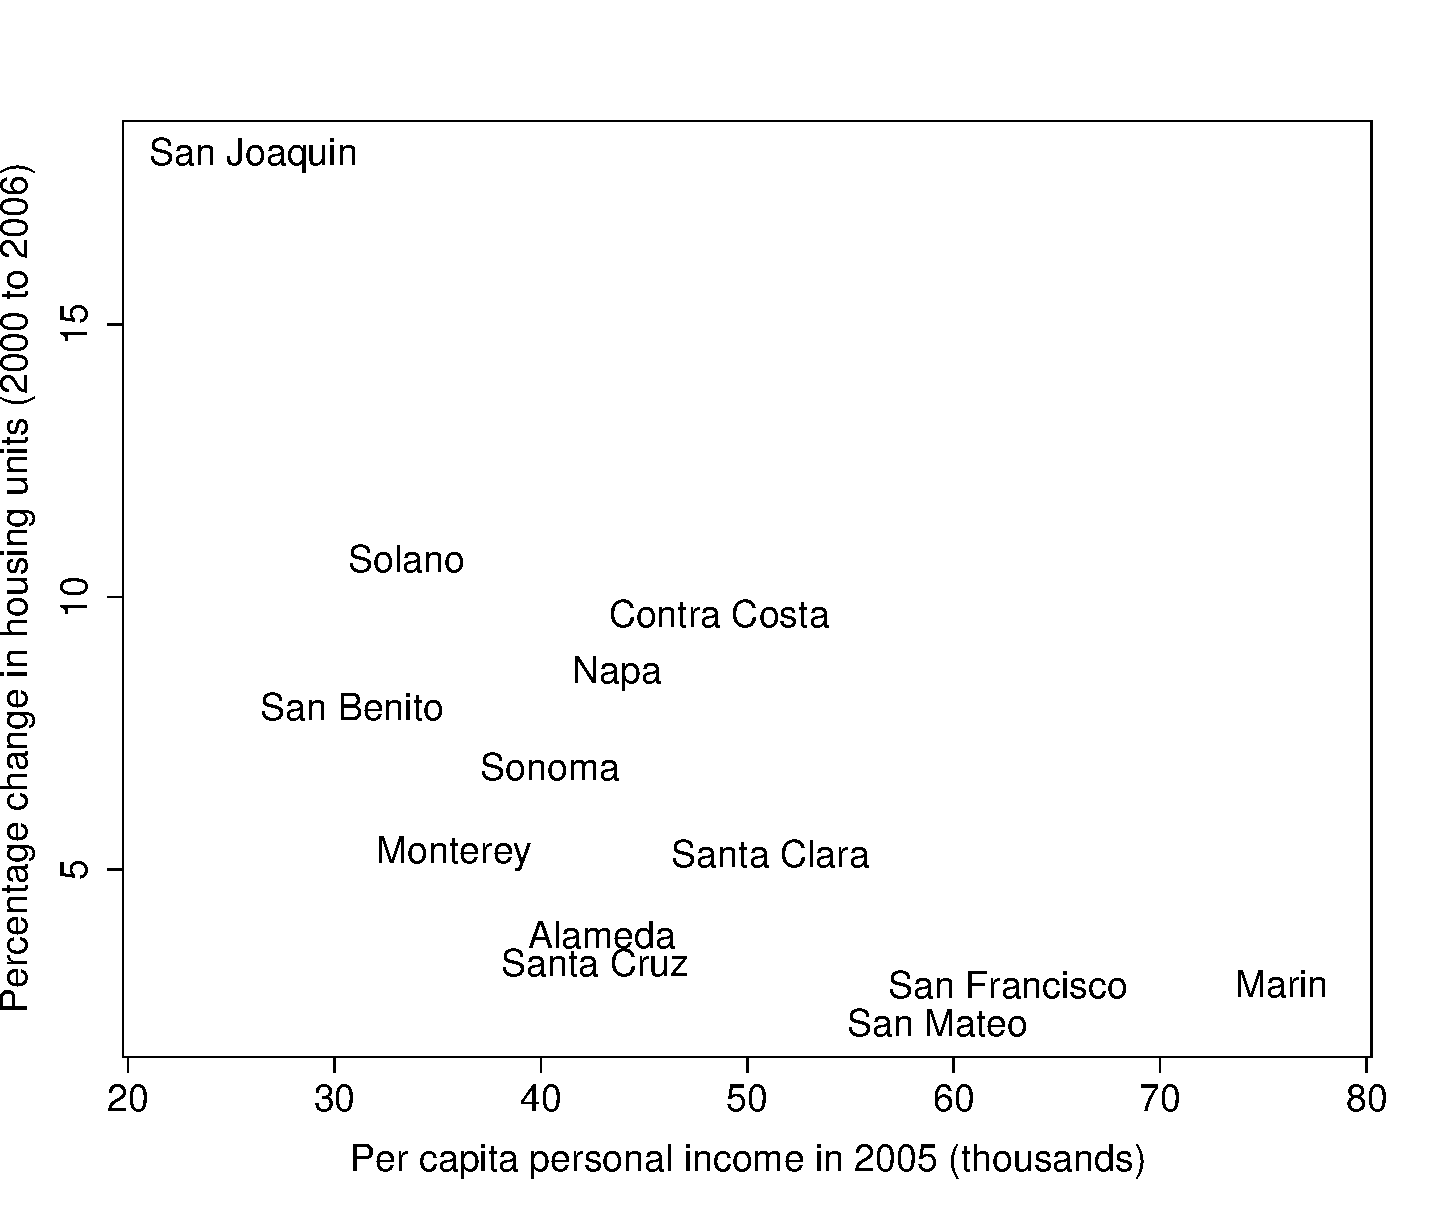
\includegraphics[width=0.5\linewidth]{county_newconstruct2}
  \caption{Relationship between new construction and recent prices (left) and personal income (right); data is aggregated by county. The relative increase in the number of housing units was greatest in towns with lower cost housing (left) and lower per capita income (right).}
  \label{fig:newconstruct}
\end{figure}

According to an article in the New York Times \citep{mckinley:2007}, the city of Stockton, one of the larger cities in San Joaquin county, already had the highest rate of foreclosures in the USA by the summer of 2007. Unfortunately we do not have any sales for Stockton prior to 2008, but it appears it was a leading indicator of the slump in the region that would continue into 2008. The population of Stockton grew rapidly in the last decade as commuters moved further out to escape the overheated housing market in the immediate Bay area. This helps to explain the new construction noted earlier, and also ties into our observation regarding commute times. The article also lists Modesto and Merced, two other towns in the Central Valley, in the top 10 nationwide for foreclosures at that time.   

%\begin{figure}[htbp]
%  \centering
%  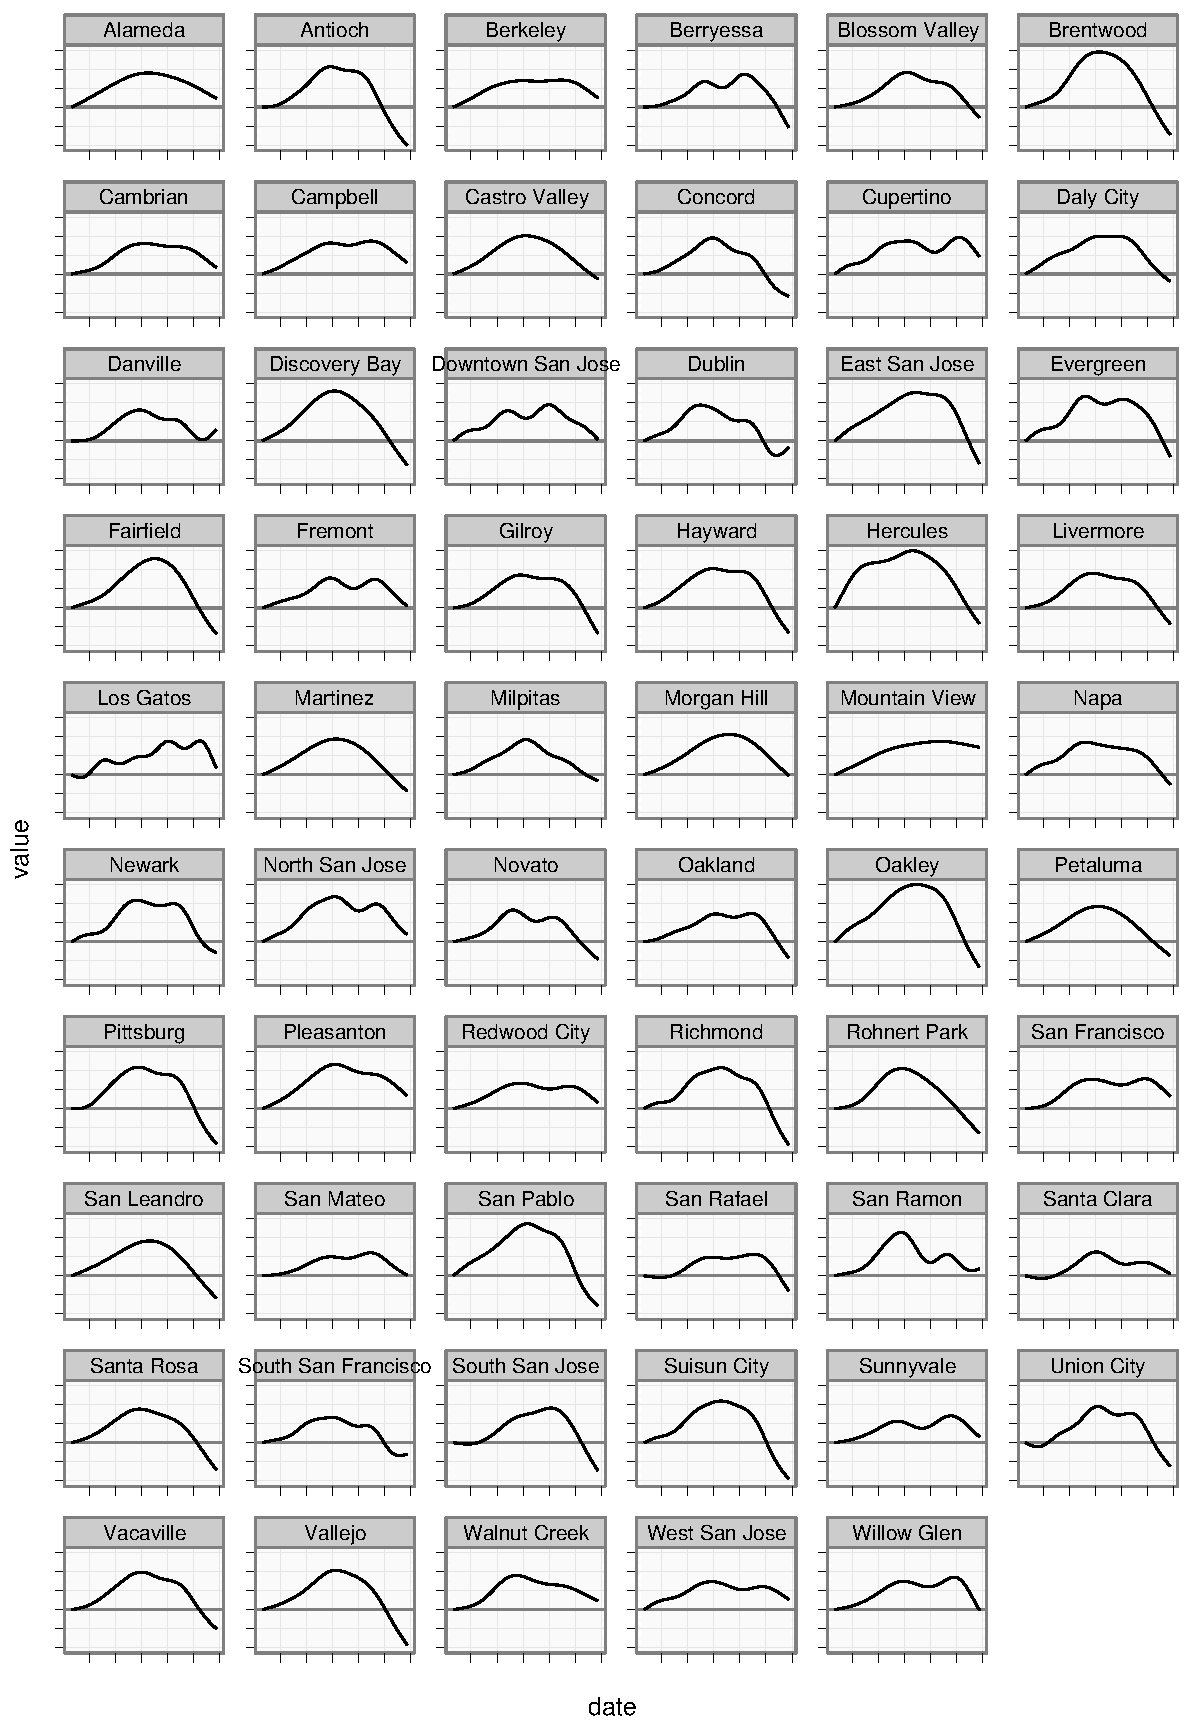
\includegraphics[width=0.9\linewidth]{cities-individual}
%  \caption{Individual plots for each city.}
%  \label{fig:individual}
%\end{figure}

\section{Exploring San Francisco}

Having explored the difference between cities, we turned to look at a single city in more detail.  San Francisco is the obvious choice:  It is the largest city in the data, it is the city with which we are most familiar, and it has some iconic features that should be easy for others to identify as well.  We started our exploration by extracting all addresses within San Francisco that were geocoded with a fairly high degree of accuracy, giving us a total of 25,377 addresses.  We created a simple scatterplot of the latitudes and longitudes, Figure~\ref{fig:sf-geo}.  For the residential parts of the city, this gives an amazingly detailed picture.  We can see the orientation of the streets, the waterfront boundaries and parks.  Our view of some areas, like downtown, is more patchy because there are fewer residential homes there.  (In this section, we will avoid using the shorthand term ``house'' since it is obvious that so many of the home sales represent apartments.)

\begin{figure}[htbp]
  \centering
  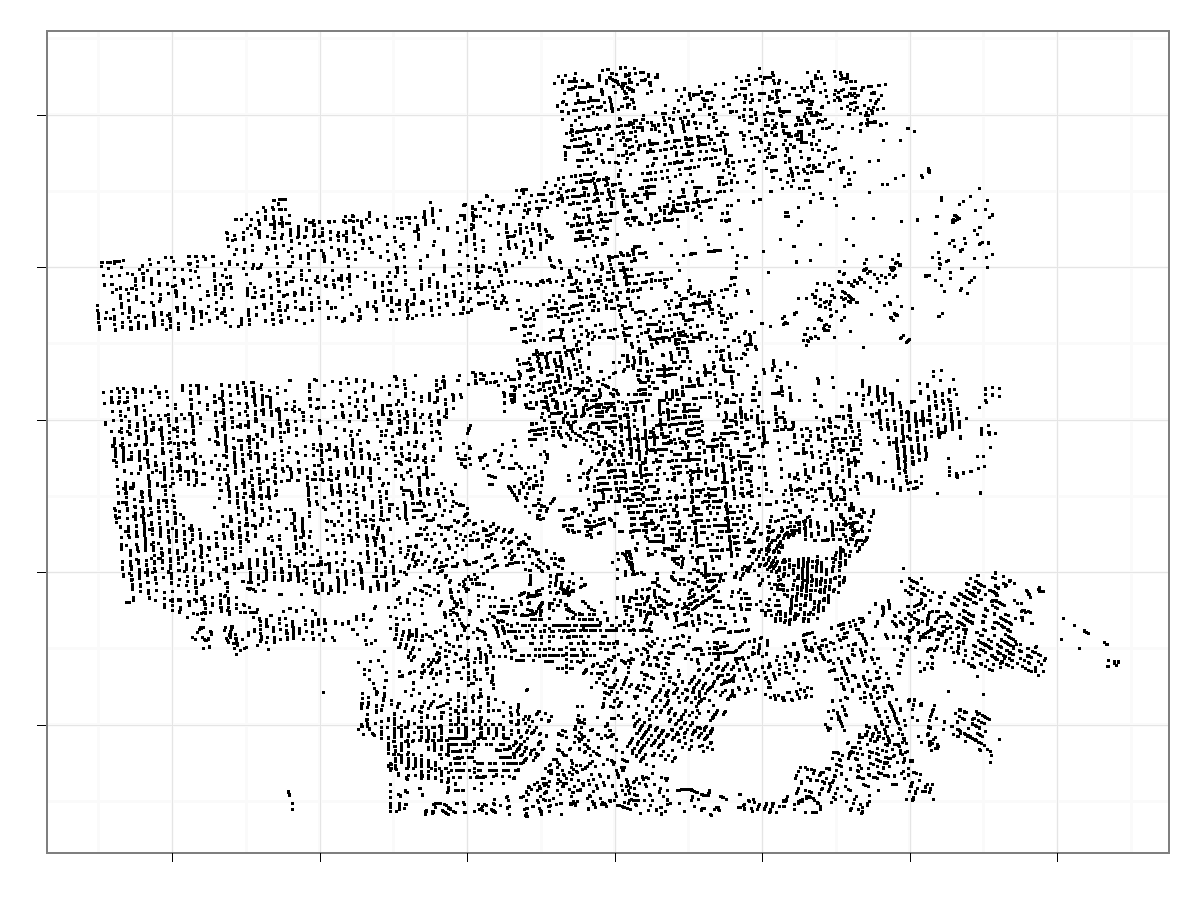
\includegraphics[height=2in]{sf-geo}%
  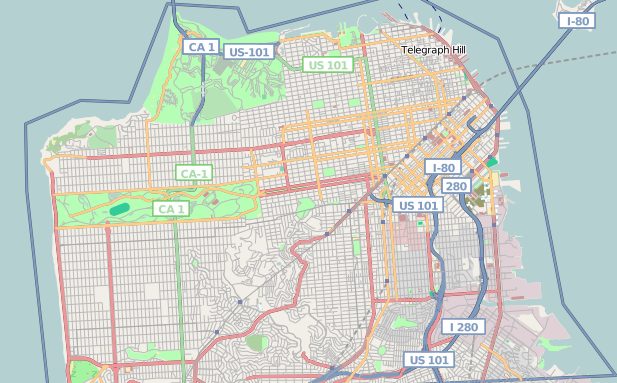
\includegraphics[height=2in]{sf-map}
  \caption{(Left) A small point is drawn for every residential sale in the data.  It gives us a pretty feel for the layout of San Francisco. (Right) For comparison, a street map of San Francisco from \url{http://openstreetmap.com}}
  \label{fig:sf-geo}
\end{figure}

One problem with this plot is we cannot see the number of sales at each specific location. Figure~\ref{fig:sf-n} shows two attempts to recapture the information. On the left, we have a bubbleplot with the size of the location proportional to the number of sales. We now get quite a different view of the downtown: there are many sales there. Looking more closely at the data reveals that these are apartment buildings with hundreds of apartments. On the right, we have divided San Francisco into squares of 0.005 latitude and longitude and counted the number of homes in each bin. This gives us a higher level view showing where the majority of homes are located.

\begin{figure}[htbp]
  \centering
    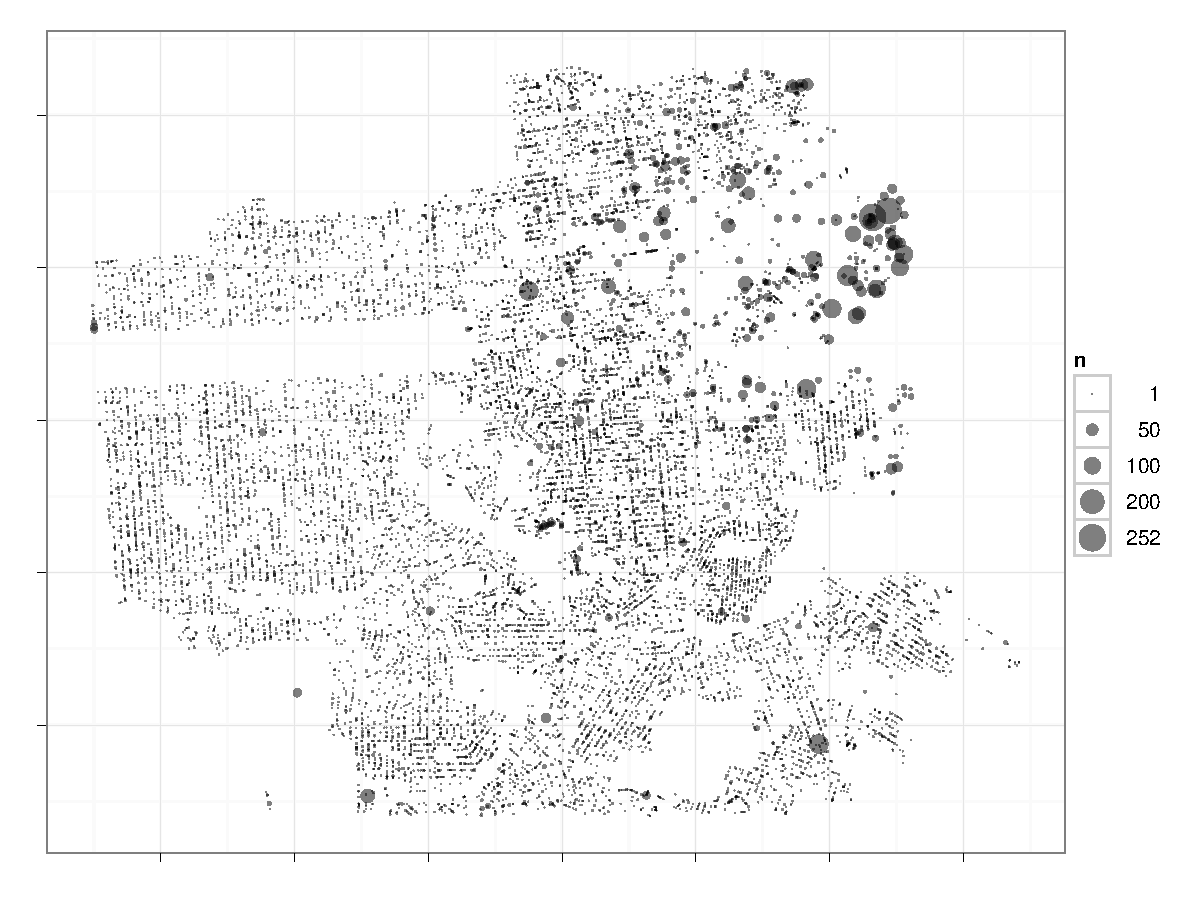
\includegraphics[width=0.5\linewidth]{sf-geo-n}%
    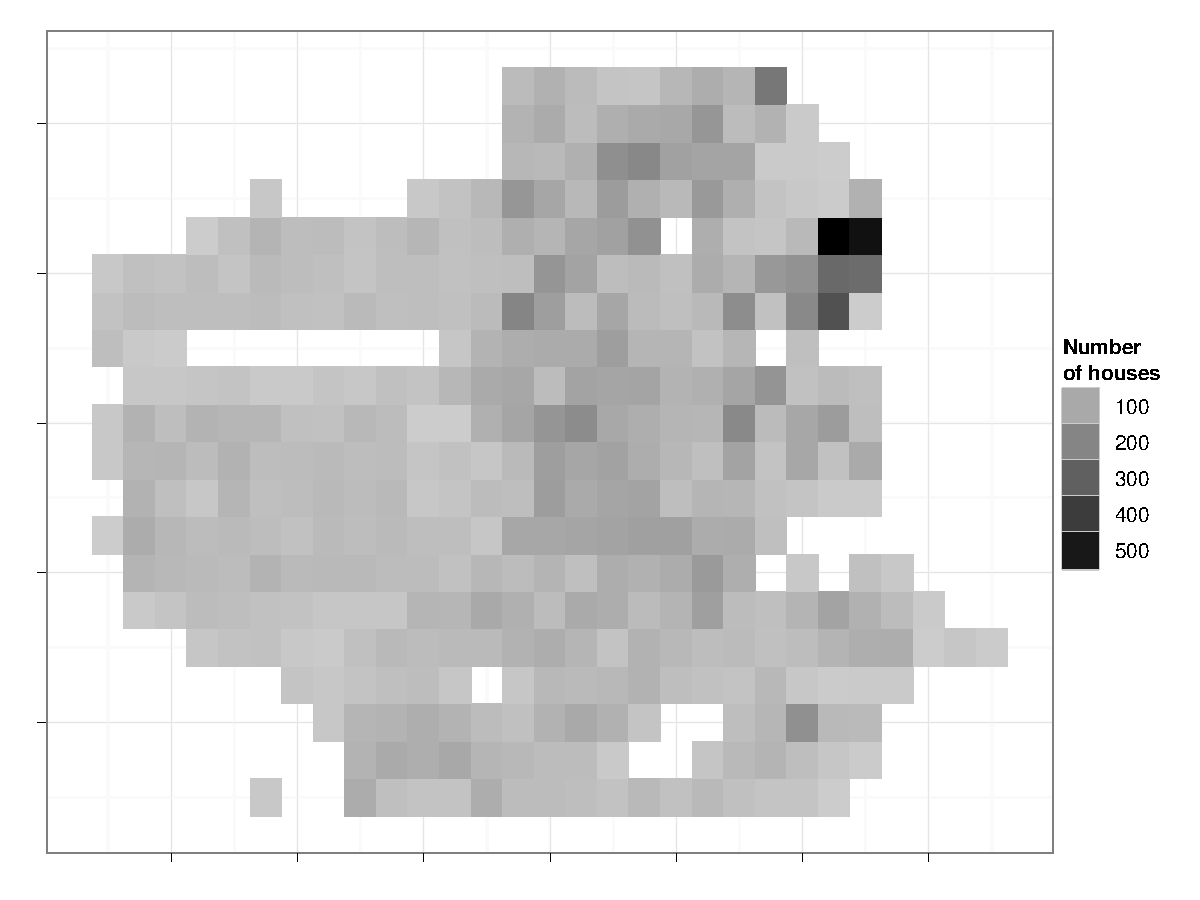
\includegraphics[width=0.5\linewidth]{sf-bin-n}
  \caption{The geographic distribution of numbers of residential sales.  (Left) this plot is similar to the previous plot, but the size of the dot is now proportional to the number of sales at each unique location.  This changes the picture significantly, as the large apartment complexes in the city now pop out.  (Right) A display of sales at a higher level of aggregation: latitude and longitude are divided into a small number of bins and the number of sales in each bin is counted and displayed as the colour of the bin.}
  \label{fig:sf-n}
\end{figure}

Using that same binning, we calculated the mean and coefficient of variation of the home prices.  The coefficient of variation is the standard deviation divided by the mean.  We use it here because a variation of \$100,000 is relatively much more important when houses are cheap compared to when they are expensive.  Figure~\ref{fig:sf-price} shows the geographic distribution of these two summary statistics.   We can see the most expensive homes border the Presidio and coast to the North of the city.  There also seems to be a peak in the Southwest - this is the affluent St. Francis Wood area, near San Francisco State University.  There is an interesting geographic trend in the coefficient of variation: it appears to increase towards the Northwest.  
%We don't know enough about San Francisco to guess as to why this occurs.

\begin{figure}[htbp]
  \centering
    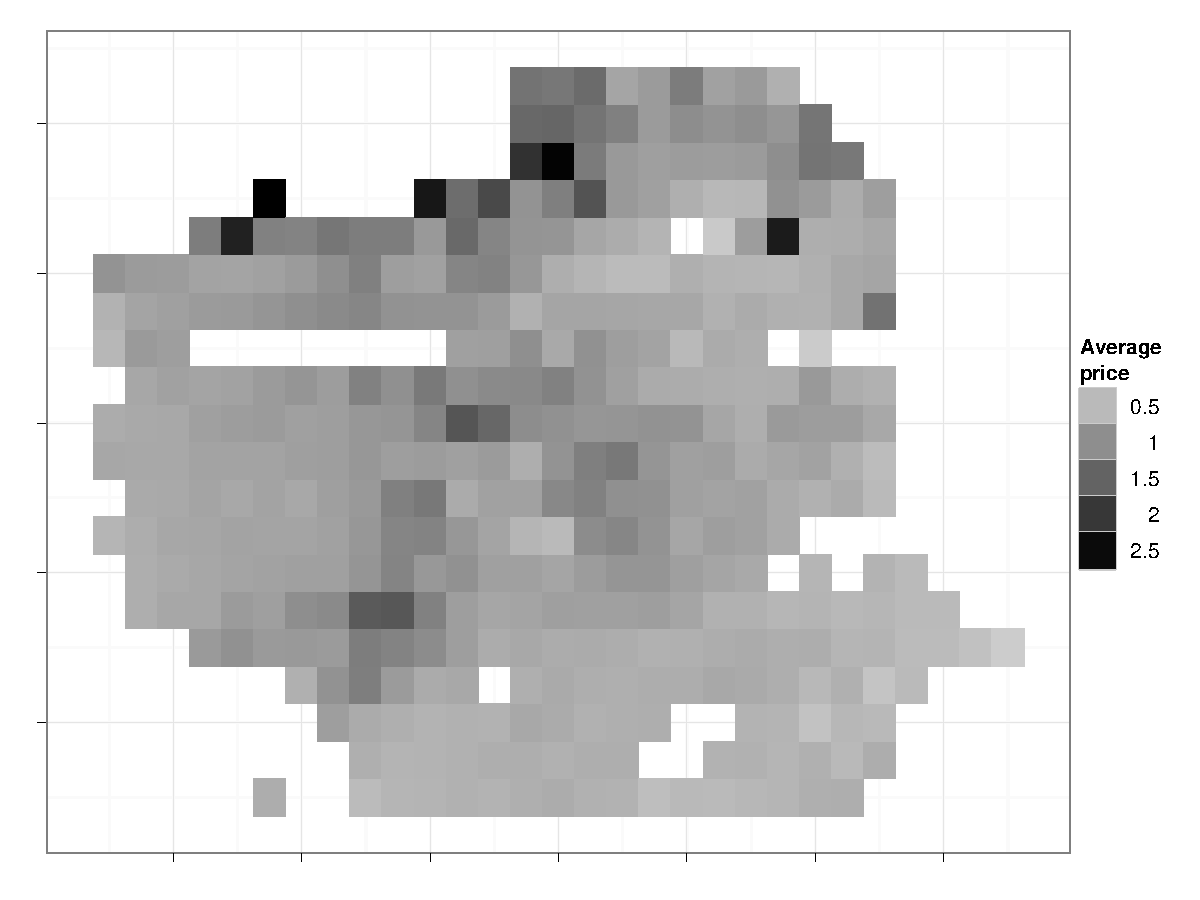
\includegraphics[width=0.5\linewidth]{sf-bin-price}%
    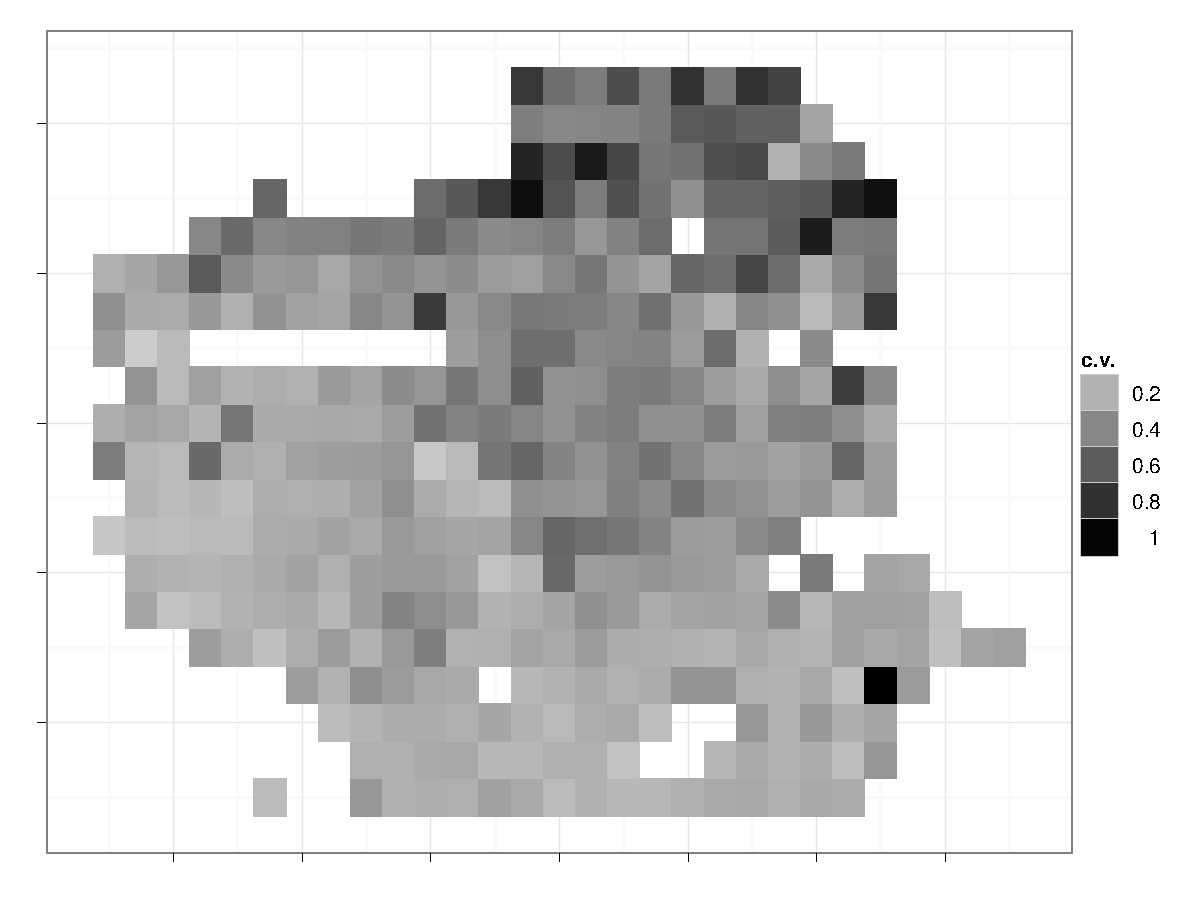
\includegraphics[width=0.5\linewidth]{sf-bin-cv}
  \caption{Geographic distribution of home prices.  Using the same binning of latitude and longitude as in the previous figure, the mean (left) and coefficient of variation (right) are computed and displayed using shades of grey.}
  \label{fig:sf-price}
\end{figure}

% We can also use this data for an unexpected purpose.  Because the data is so dense and includes the year that the home was built, we can explore historical patterns of housing development.  This idea was inspired by truliaHindsight, \url{http://hindsight.trulia.com/}, but because we have the data in an unencumbered form we are much freer to experiment with the visualisation of this data.  They have much more data, 150,000 vs 27,000, but we can display more (they display at most 2000 points at once), and we can do more sophisticated analyses.

\section{Conclusions}

 % Both code and data are licensed with the permissive MIT license.  We'll illustrate snippets of code and fragments of the data inline, but each section of this chapter will also point you to a matching file online.  The files don't cover the exactly content as each section: you can see some of the dead ends we tried, and some of the plots that weren't quite good enough to make it into the plot.  
 % 

We have looked at the data from several angles, and we have been consistently led to same conclusion: The housing crisis has been relatively more damaging in poorer areas.  Both the boom and the bust hit lower-priced homes earlier.  A great deal of the boom was associated with new construction, most of which was aimed at the lower end of the market.  Many of the new residences were built farther from San Francisco, in less developed areas where residents had lower average incomes, more children, and longer commutes.  The bust hit earlier and harder at the low end, too.  Although the biggest absolute decline in prices occurred at the high end, it was the less expensive houses that lost a greater percentage of their value.  

All of this is consistent with what we have learned about sub-prime mortgages since the housing bust entered the headlines.  Many people with poor credit were granted mortgages with initially low monthly payments; when those payments grew, they were unable to meet them, and the rates of mortgage defaults and foreclosures began to rise.  We speculated earlier that the increase in sales in 2008 may be associated with foreclosures, and an interesting next step would be to locate data on foreclosures and align it with our sales data.

We have used relatively simple statistical methods such as indexing, computing quantiles, smoothing and binning to explore a large and complex data set.  We began with broad summaries and then dug deeper to explore the details, but we have only scratched the surface.  If the data has caught your interest and you'd like to follow our work in more detail, or try out some your own ideas, you can find all data and code in a repository at \url{https://github.com/hadley/sfhousing}.  All the tools we used are open source, so anyone should be able to replicate our work. The principle of reproducibility \citep{gentleman:2007} so critical in the laboratory sciences can be extended to this kind of analysis.  If we made a mistake, someone else should be able to discover it, fix it and observe the effects on our conclusions.  

[ Shall we list our tools?  Don't know. 
(linux, MacOS X are trademarked, so we'd need footnotes)]

Tools: shell (wget, awk,); perl; R (ggplot2, plyr, reshape).

%The creation of a reproducible data analysis can be a lot of extra work, but once the principles are ingrained in the workflow, it doesn't take that much time.  Importantly, it is not only useful for others, but also to the original analyst, who in time will likely forget the finer details of the work. A well-commented reproducible analysis will save a lot of time when revisited later.
%If you haven't made your analysis reproducible and you come back to it 6 months or a year later (quite common if you are submitting the results to an academic journal), you may look at the code and wonder what on earth you were thinking. If you have made the analysis reproducible and included plenty of comments about your thinking, then you save a lot of time trying to reproduce your previous work and state of mind. It also very useful if your data changes.    In our case, we updated just before writing up the paper so that we had the latest data off the website.  Data changes a lot more than you might think.  Even when your data is about something that has already happened, often the data will change  as errors are discovered and fixed.  Every statistician has a story about a nightmare client whose data would not stay the same from week-to-week.

%Another tool that we find useful is source code control.  In an analogous way to software development, this makes it easy to discard parts of the analysis that led nowhere or have been superseded.  The code on the repository website indicates that (by and large) the analysis follows a fairly logical flow.  This is not how it starts off!  Data analysis is a fairly creative process, with many blind alleys, mistakes and alternative approaches.  Inclusion of all of these makes it hard to follow exactly what we did, but removing them completely makes it hard to see all the things that we tried.  
%Using a code versioning system leaves us with a happy medium where the false paths are not immediately visible, but can be looked up (although current tools are somewhat lacking for this purpose).

We enjoy working with data, exploring and learning from it.  We hope we have shared with you our enthusiasm for data analysis, and have shown you some of the tools and techniques that we find most useful.

% Tools: shell (wget, awk,); perl; R (ggplot2, plyr, reshape).

% Note about graphics: can churn out rough versions for exploration very quickly - takes more time to polish them for publication.  Clarify story, remove extraneous elements and ensure that it supports the text.

% A little tricky because working on this data analysis also lead us to develop some new tools, and it takes some time for these to trickle into released versions.  If you have problems running the code we released, please let us know!  Data analysis like software development.  Local caches to speed things up and to provide some backup if the original sources go down.

% Tension with interactive tools: they are great for discovery, but bad for reproducibility.  Once you have discovered something in your interactive tool, you need to be able to reproduce it independently so that others can see it too.  Area of active research (cite Heer's work).  



% bibtool -x beautiful-data.aux > references.bib
\bibliography{references}

\end{document}
